% Hier können die einzelnen Kapitel inkludiert werden. Sie müssen in den 
% entsprechenden .TEX-Dateien vorliegen. Die Dateinamen können natürlich 
% angepasst werden.

% TODO: Was ist mit der geführten Tour? Aus Lasten/Pflichtenheft und allem komplett raus? Oder im Flietext mit einbringen zB beim Lasten, Pflichtenheft?
% TODO: Administrationstabelle fällt raus aus ERM, Lastenheft, Pflichtenheft -> Alles über HTTP BasicAuth


\section{Einleitung}
\label{sec:Einleitung}
Für viele Menschen stellt das Internet in der heutigen Zeit das wichtigste
Medium zur Informationsgewinnung dar. Durch die Entwicklung des Internets hin
zum Web 2.0 werden dem Nutzer immer neue Möglichkeiten geboten, auf das
umfassende Angebot an Informationen im Internet zuzugreifen. Der Zugriff auf
dieses Informationsangebot gestaltet sich hierbei zunehmend interaktiver.
Diese Interaktivität wird immer häufiger auch von Unternehmen genutzt.
Unternehmen präsentieren sich nicht mehr nur auf der firmeneigenen
Internetseite, sondern betreiben Marketing in sozialen Netzwerken,
veröffentlichen Neuigkeiten in Blogs und aquirieren neue Mitarbeiter über
Internetplatformen. Der Trend hin zur Nutzung dieser modernen
Kommunikationsmittel zeigt, dass es hiermit möglich ist weltweit eine große
Zielgruppe anzusprechen und auf sich aufmerksam machen zu können.

Im Rahmen des Projektes "`Virtueller Campus Lingen"' sollen diese neuen
Möglichkeiten der Internetpräsenz auch für den Standort Lingen der Hochschule
Osnabück nutzbar gemacht werden. Hierbei soll der neue Campus des
Studienstandorts Lingen einer breiten Masse an Studieninteressierten
präsentiert werden.

Bei der Durchführung eines Projektes von diesem Ausmaß ist es wichtig die
Komplexität handhabbar zu machen und das Projekt möglichst genau zu planen,
steuern und kontrollieren zu können. In dieser Ausarbeitung soll aus diesem
Grund die Vorgehensweise bei der Auftragsfindung, der Konzeptionierung,
Umsetzung und Reflexion des Projektes "`Virtueller Campus Lingen"' aus Sicht der
Unternehmensführung dargestellt werden. Zunächst wird im Abschnitt
"`Projektauftrag"' die Projektidee, sowie das Projektumfeld und die Projektziele
herausgestellt. In den Projektzielen wird hierbei der Nutzen des Projektes
für den Auftraggeber verdeutlicht. Auf den Projektautrag aufbauend soll
die Entwicklung des Projektkonzeptes im Abschnitt "`Konzeptionierung"'
beschrieben werden. Nachfolgend werden die für die Umsetzung des Projektes
benötigten Ressourcen Zeit und Kosten geplant. Anschließend werden im Abschnitt
"`Projektdurchführung"' sowohl die Organisation der Projektgruppe als auch die
einzelnen Phasen, in denen das Projekt durchgeführt wurde, erläutert.  

In der darauffolgenden Projektreflexion werden geplante und benötigte Ressourcen
in einem Soll-Ist-Vergleich gegenübergestellt und die Erreichung der zuvor
aufgestellten Projektziele verifiziert. Für den Auftraggeber werden hier die
angefallenen Kosten den erreichten Projektzielen und somit dem Nutzen des
Projektes gegenübergestellt. Weiterhin werden die subjektiven Eindrücke der
Projektmitglieder im Bezug auf die Kommunikation, das Verhalten in der Gruppe
und die Betreuuung der Arbeit durch die Dozenten reflektiert. Nach der
Reflektion wird ein Ausblick auf eine mögliche Weiterführung des Projektes
gegeben. Abschließend wird von der Projektgruppe eine Handlungsempfehlung
bezüglich der Veröffentlichung und Erweiterung des Projektes an den Auftraggeber
ausgesprochen.
\section{Architekturgrundlagen}
\label{sec:Architekturgrundlagen}

Das vorliegende Projekt beschreibt die Entwicklung einer Softwarelösung für das im Vorfeld beschriebene Problem.
Im Zuge dieser Entwicklung wird eine Architektur entwickelt, die auf verschiedenen Technologien aufbaut.
Das nachfolgende Kapitel dient dazu diese Technologien grundlegend zu erläutern, um deren weitere Verwendung
nachvollziehen zu können. Zu diesem Zweck wird die entwickelte Architektur im folgenden Schaubild (\abbildung{Architektur}) vorausgestellt.
Die Entwicklung dieser Architektur wird aufbauend auf den folgenden Grundlagen in den nachfolgenden Kapiteln beschrieben.

\begin{figure}[htb]
\centering
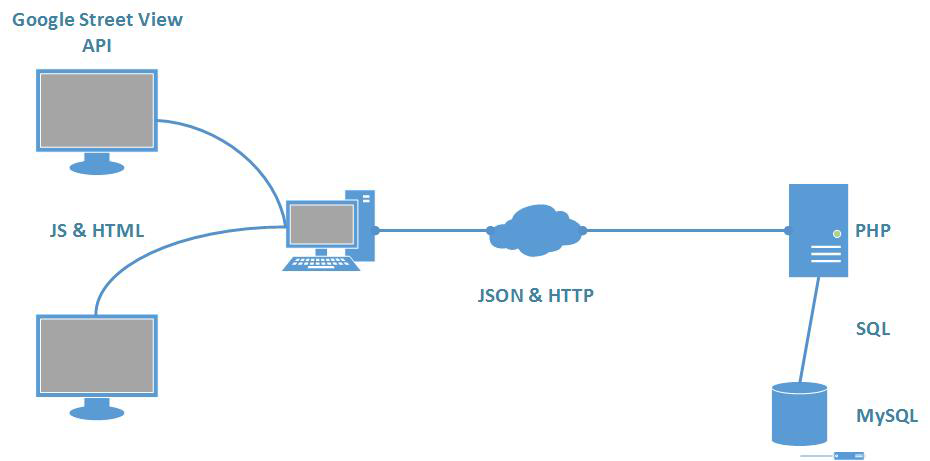
\includegraphics[width=1.0\textwidth]{Architektur.png}
\caption[Architektur der Anwendung]{Architektur der
Anwendung\protect\footnotemark}
\label{fig:Architektur}
\end{figure}
\footnotetext{Quelle: Eigene Darstellung}


In diesem Architekturentwurf ist die Verwendung von vier Technologien vermerkt. Diese sind:
\begin{itemize}
  \item HTML
  \item Javascript
  \item PHP
  \item SQL
\end{itemize}

Diese Technologien sind grundlegend für das Verständnis der entwickelten Software.
Aus diesem Grund werden die wichtigsten Grundlagen zu jeder Technologie nachfolgend erläutert.
Der Fokus liegt dabei immer auf den Teilbereichen, die im vorliegenden Projekt eingesetzt werden.
\subsection{HTML}
\label{sec:Html}

Die Hypertext Markup Language, abgekürzt HTML, stellt eine deklarative Sprache zur Beschreibung und Gestaltung von Internetseiten dar. Die erste Spezifikation von HTML erschien 1989, wobei sich die Spezifikation im Laufe der Zeit verändert und erweitert haben\footnotetext{\citet{taglinger2003}}.

Mithilfe von HTML können Dokumente erstellt werden, welche von Internetbrowsern gelesen, interpretiert und dem Inhalt entsprechend dargestellt werden. Dargestellt werden können Text, Bilder, Tabellen, Verlinkungen, Videos usw.

Der grundlegende Aufbau von HTML erfolgt hierbei durch sogenannte Tags, wobei die meisten Befehle einen Start- und einen Endtag besitzen.
Das Tag <html> dient zur Öffnung eines HTML-Bereichs, welcher die weiteren Bereiche und Inhalte für die Darstellung einer Internetseite besitzt. Dieses Tag und das gesamte Dokument werden zum Schluss mit dem Tag </html> geschlossen. Das Tag <head> enthält Kopfdaten, z.B. den Titel einer Internetseite, welcher in der Kopfzeile des Internetbrowser angezeigt wird. Im <body>-Bereich des HTML-Dokuments, welcher ebenfalls mit einem Tag geschlossen werden muss, wird der eigentliche Inhalt der Internetseite angegeben. Dieser wird dann im Browserfenster entsprechend den Angaben und Inhalten dargestellt.
Die Struktur eines stellt sich somit folgendermaßen dar:

%TODO: Listing erstellen

% <html>
% <head>
% <title>Titel der Internetseite </title>
% </head>
% <body>    Inhalt der Internetseite
% </body>
% </html>

Im vorherigen Beispiel würde somit eine Internetseite im Browser angezeigt werden, welche den Titel "`Titel der Internetseite"' in der Kopfzeile anzeigen würde. Als Inhalt würde nur der Text "`Inhalt der Internetseite"' angezeigt werden, ohne jegliche zusätzliche Formatierungen.

Die neueste Spezifikation von HTML, HTML5, bietet einige nützliche Erneuerungen, so können nun unter anderem direkt im HTML-Dokument Audio oder Videodateien eingebunden werden, ohne das zusätzliche Plugins, wie z.B. Adobe Flash benötigt werden, um diese abspielen zu können.
\subsection{Javascript}
\label{sec:Javascript}
\subsection{PHP}
\label{sec:Php}

PHP (Hypertext Preprocessor) ist eine serverseitige Skriptsprache, die mit dem Ziel entwickelt wurde Webseiten dynamisch
zu gestalten.
Mit dieser Intention wurde auch im vorliegenden Projekt PHP als Serversprache verwendet. Die nachfolgend beschriebenen
Grundlagen vermitteln die wichtigsten Aspekte der Sprache PHP, die nötig sind, um die Umsetzung des Projektes
nachvollziehen zu können.
Im Gegensatz zu der vorher beschrieben Skriptsprache Javascript ist PHP eine serverseitige Skriptsprache. Dadurch sind
zwei grundlegende Unterschiede zu Javascript bedingt:

\textbf{1}. PHP wird, wie die Beschreibung Serverskriptsprache bereits suggeriert, nicht auf dem Client (dem Browser des Nutzers),
sondern auf dem Webserver der Anwendung ausgeführt. Bei einer Nutzeranfrage an den Webserver wird also erst eine PHP-Routine serverseitig ausgeführt und anschließend wird das angefragte Dokument, inklusive
Javascriptdateien, an den Client (Browser) ausgeliefert und dort wird dann Javascript ausgeführt.

\textbf{2}. PHP hat weitestgehend vollen Ressourcenzugriff auf dem ausführenden System. Durch PHP-Befehle ist es zum Beispiel möglich Dateien auf dem ausführenden System (Webserver) anzulegen und zu löschen.
Diese beiden Unterschiede sind wichtig, um das Einsatzfeld von PHP zu verstehen.

PHP wird im vorliegenden Projekt für die folgenden Aufgaben eingesetzt:
\begin{itemize}
  \item Kommunikation mit der Datenbank
  \item Schreiben von dynamischen HTML
  \item Kopieren von Benutzerdateien auf das ausführende System.
\end{itemize}

Diese Aufgaben werden im späteren Verlauf ausführlicher beleuchtet, an dieser Stelle soll die Listung dieser Aufgaben
ausreichen, um ein Verständnis für die Einsatzfelder von PHP zu bekommen.
Um diese Aufgaben zu erfüllen sind in PHP, wie in jeder anderen Programmiersprache auch, Befehle mit einer vorgebenen
Syntax definiert. Diese Befehle werden im Quellcode in einem besonders gekennzeichneten Bereich geschrieben. Dieser
Bereich wird durch die Zeichenfolge '<?php' eingeleitet und mit der Zeichenfolge '?>' beendet.
Abschließend soll die folgende Abbildung die Anwendung von PHP verdeutlichen:

\lstinputlisting[language=PHP,caption={PHP Grundlagen},label={lst:PHP Grundlagen}]{Listings/PHP_Grundlagen.php}

In diesem Beispiel wird die Anfrage eines Benutzers ausgewertet. Die eigentliche Anfrage ist dabei nebensächlich und aus diesem Grund nicht dargestellt (auskommentiert in Zeile 2). Die Auswertung der Anfrage soll an dieser Stelle zeigen auf welchem Weg mit Hilfe von PHP dynamisches HTML geschrieben werden kann. In dem dargestellten Beispiel wird die Benutzeranfrage ausgewertet und je nachdem, was diese Anfrage zurückliefert wird ein HTML p-Tag mit anderem Inhalt geschrieben. Im Browser des Benutzers würde dadurch ausgegebn, ob seine Anfrage positiv oder negativ ausgewertet wurde.
\subsection{Datenbanken und SQL}
\label{sec:DatenbankenUndSql}

Eine Datenbank ist das Rückgrat jedes datenverarbeitenden Informationssystems. Dementsprechend häufig sind Datenbanken in 
verschiedenen Kontexten anzutreffen (Web-, ERP-, Mobile-Systeme, etc.). Die nachfolgende theoretische Fundierung dient zum 
Verständnis des Einsatzes der Datenbank im vorliegenden Projekt.

"`Eine Datenbank ist eine Sammlung von Daten, die einen Ausschnitt der realen Welt beschreibt."'\footnote{\citet{elmasri2009}}
Diese
Sammlung von Daten kann dabei sowohl in Papierform, als auch elektronisch und computergestützt aufbewahrt werden. Vor dem 
Hintergrund des vorliegenden Projektes gilt die weitere Betrachtung aber ausschließlich den computergestützten Datenbanken.
In diesem Teilbereich gibt es wiederum verschiedene Datenbanktypen, die sich in der Verwaltung und Haltung der Daten 
unterscheiden. Die wichtigsten Datenbanktypen sind im Folgenden aus Gründen der Abgrenzung aufgelistet:

\begin{itemize}
  \item hierarchische Datenbanken
  \item objektorientierte Datenbanken
  \item relationale Datenbanken
  \item NoSql Datenbanken
\end{itemize}

Der Fokus dieser Spezialisierung liegt im Folgenden wiederum auf der eingesetzten Technologie des Projektes und damit auf 
relationalen Datenbanken. 

Eine relationale Datenbank beruht auf dem relationalen Datenbankmodell von Edgar F. Codd aus dem Jahre 1970.\footnote{siehe dazu \citet{codd1970}} Grundlage dieses Modells ist der Begriff der Relation, der im Wesentlichen
eine mathematische Beschreibung einer Tabelle darstellt. Eine relationale Datenbank ist damit eine Sammlung von Tabellen.

Auf den Relationen (Tabellen) einer solchen Datenbank sind bestimmte Operationen definiert, die im Kontext der Mathematik 
der relationalen Algebra und im Kontext von Datenbanken dem Begriff SQL entsprechen.

SQL steht für Structured Query Language und stammt, genau wie das relationale Datenbankmodell, aus dem Jahre 1970. Es 
wurde ebenfalls von Edgar F. Codd mitentwickelt.\footnote{\citet{kline2005}} Über einen Entwicklungszeitraum von mehreren Jahrzehnten 
wurde SQL zu einer komplexen Sprache, die umfangreiche Möglichkeiten bietet. Dieser Gesamtkomplex wird hier stark verkürzt
dargestellt und beschränkt sich nur auf die wesentlichen Aspekte, die dem Verständnis des Projektes dienen.

SQL dient im Wesentlichen zum Definieren, Kontrollieren und Manipulieren von Datenstrukturen. Um diese 
Bereiche zu trennen sind in SQL drei Sprachbereiche definiert.

\begin{description}
  \item[Data Definition Language (DDL)] dient zum Erstellen, Löschen und Ändern von Tabellen.
  \item[Data Control Language (DCL)] dient zum Vergeben und Entziehen von Berechtigungen.
  \item[Data Manipulation Language (DML)] dient zum Lesen, Schreiben, Löschen und Ändern von Datenstrukturen.
\end{description}

Die Sprachbereiche DDL und DCL haben dabei in der Projektentwicklung eher einmaligen Charakter, wohingegen DML 
kontinuierlich verwendet wird, um dynamisch Informationen zu schreiben oder zu lesen. Die DML tritt dabei als 
Schnittstelle zwischen Anwendungsprogramm und Datenbank auf (siehe Abbildung: \nameref{fig:Architektur}). Über die DML sind beispielsweise 
Befehle definiert, die es erlauben einen Datensatz einer Tabelle zu lesen oder zu verändern. Diese Befehle werden im 
Anwendungsprogramm aufgerufen und erzeugen damit dynamischen Inhalt für den Anwender.
\section{Analyse und Planung}
\label{sec:AnalyseUndPlanung}

% TODO: Verweis auf andere Ausarbeitung einbinden. 2x
Nach der Fundierung der Architektur Grundlagen wird die enstehende Softwarelösung geplant. Es wird angesetzt am 
entwickelten Konzept (siehe Ausarbeitung Unternehmensführung) des Projektes und an der daraus resultierten Problemlösung 
(siehe Ausarbeitung Unternehmensführung). Darauf aufbauend wird zunächst eine Analyse der Ist-Situation vorgenommen. 
Hierraus geht hervor, ob es in der Ist-Situation der Hochschuldarstellung Elemente (anderes Wort finden) gibt, die für die 
neue Softwarelösung wiederverwendet werden können. Die Planungsphase wird beendet mit der Definition der Anforderungen in 
Form eines Lastenheftes und der Festlegung der Projektgrenzen.
\subsection{Ist-Analyse}
\label{sec:IstAnalyse}

Momentan lassen sich Informationen über die angebotenen Studiengänge am Studien-
standort Lingen über die Hochschulseite www.hs-osnabrueck.de abrufen. Die Internetseite bietet dabei zum einen 
weiterführende Links zu den einzelnen Instituten und darüber auch viele Informationen für Unternehmen und Studierende.
Hier werden zum Beispiel Labore, Projekte und Dozenten der einzelnen Institute vorgestellt. Zum anderen werden in einer 
Bildergalerie einzelne Impressionen des neuen Campus dargestellt. Ein Screenshot hiervon ist in \abbildung{Bildergalerie} abgebildet.

\begin{figure}[htb]
\centering
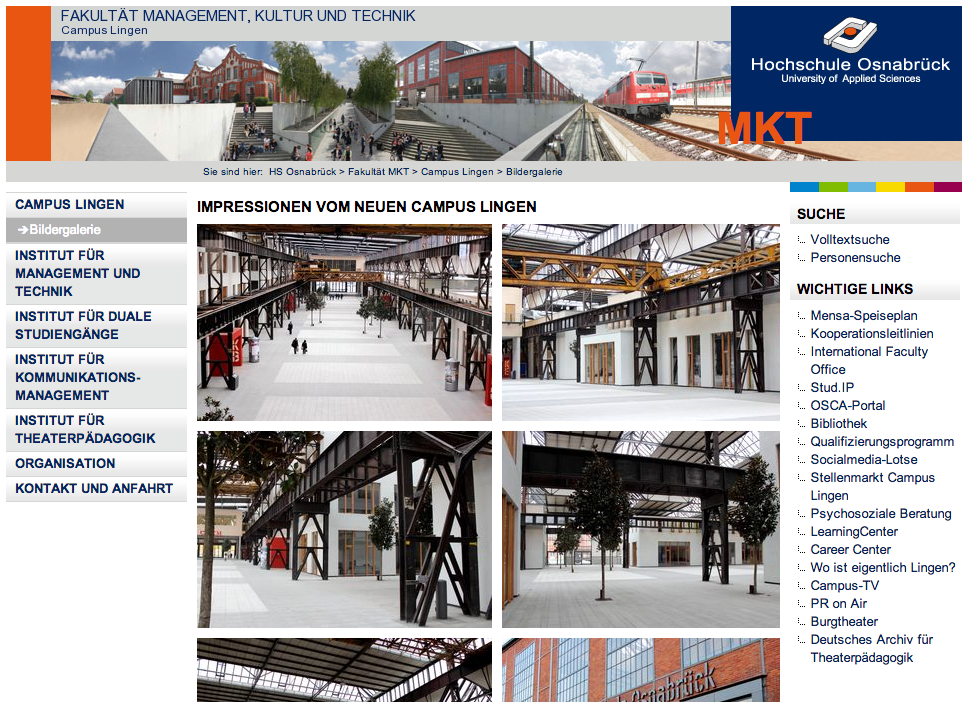
\includegraphics[width=1.0\textwidth]{Bildergalerie.png}
\caption[Bildergalerie des Campus Lingen]{Bildergaliere des Campus Lingen\protect\footnotemark}
\label{fig:Bildergalerie}
\end{figure}
\footnotetext{Link: http://www.campus-lingen.hs-osnabrueck.de}

Ähnlich wie die Informationsvermittlung auf der Internetseite der Hochschule Osnabrück
gestaltet sich auch die Informationsvermittlung auf Messen, auf denen Studieninteressierte
sich auch über die einzelnen Studienstandorte erkundigen können. Dort werden ebenfalls
Impressionen des Campus in Lingen gezeigt oder Informationsmaterial verteilt.

Vor dem Hintergrund der Projektidee, den Campus in 360-Grad Panoramas mit Informationstexten abzubilden, bilden sich aus 
dieser Analyse 2 interessante Elemente heraus.

\textbf{1.} Die Fotos, die bereits vom neuen Campus gemacht wurden.

\textbf{2.} Das Informationsmaterial das über Projekte, Studiengänge, Dozenten und weiteres zusammen getragen wurde.

Die bereits angefertigen Fotos können dabei nicht für das vorliegende Projekt verwendet werden, da es sich bei diesen 
Fotos nicht um 360-Grad Panoramafotos handelt. Darüber hinaus sind auf diesen Fotos nur einzelne Impressionen des Campus 
dargestellt. Das bedeutet die bestehenden Fotos müssten um neu angefertigte ergänzt werden und das ist aus Gründen 
unterschiedlicher Lichtverhältnisse kein sinnvolles Vorgehen. Die bestehenden Impressionen zeigen aber
interessante Blickwickel des Campus. Diese Blickwinkel können bei der Erstellung der neuen Fotos aufgegriffen werden. 

Das zusammengetragene Informationsmaterial kann dagegen aus der Internetquelle der Hochschule verwendet werden, um 
Informationen zu bestimmten Panoramas anzuzeigen. Für die Rechereche nach Informationsmaterial muss daher kein weiter 
Aufwand im Projekt berücksichtigt werden.
\subsection{Lastenheft}
\label{sec:Lastenheft}

% TODO: Verweis auf Unternehmensführung richtig machen
% TODO: Lastenheft hier und im Original überarbeiten!!!!
Nach der Analyse der Ist-Situation gilt es im Folgenden das konkrete Ziel und die Funktionen des Projektes zu definieren. 
Zu diesem Zweck wurde aufbauend auf der Konzeptentwicklung (siehe Kapitel XX Ausarbeitung Unternehmensführung) ein 
Lastenheft angefertigt\footnote{siehe \citet{lastenheft2013}}.

Im Lastenheft ist das folgende Ziel für das vorliegende Projekt definiert:

"`Ziel des Projektes Virtueller Campus Lingen ist es den Standort der Hochschule Osnabrück
in Lingen virtuell darzustellen sowie alle vier Institutionen mit ihren Studienangeboten
vorzustellen."' \footnote{\citet{lastenheft2013}}
Die Darstellung des Campus soll dabei im Stile von Goole Street View\copyright\ in 360-Grad Panoramafotos erfolgen, in 
denen sich ein Nutzer der Software frei umsehen kann. Darüber hinaus soll ein Backendsystem zur Pflege und Wartung der 
Software entwickelt werden\footnote{\citet{lastenheft2013}}.

Zur Erfüllung der Zielbestimmung des Lastenheftes sind darin folgende Produktfunktionen definiert:

\textbf{Benutzerfunktionen}:

\begin{description}
  \item[LF0010] Einem beliebigen Internetnutzer muss es möglich sein, ohne Anmeldung auf die Anwendung zugreifen zu können.
  \item[LF0015] Beim Starten der Anwendung soll dem Benutzer ein 360-Grad Panorama vom Eingangsbereich des Campus Lingen 
  präsentiert werden.
  \item[LF0020] Der Benutzer muss sich in den 360-Grad Fotos der Anwendung frei umsehen können.
  \item[LF0030] Der Benutzer muss zwischen den Fotos navigieren können.
  \item[LF0040] Die Anwendung muss eine Übersichtkarte enthalten, die sowohl den aktuellen Standpunkt, als auch alle 
  weiteren Einstiegspunkte umfasst.
  \item[LF0050] Die Übersichtskarte stellt alle Gebäude des Campus Lingen in Vogelperspektive dar. Innerhalb der 
  Übersichtskarte sind alle Einstiegspunkte in die 360-Grad-Ansicht enthalten.
  \item[LF0060] Die Minimap soll in der oberen linken Ecke des 360-Grad-Fotos angezeigt werden.Sie stellt einen Ausschnitt 
  der Übersichtskarte dar.
  \item[LF0070] In den 360-Grad-Fotos müssen relevante Informationen zu den dargestellten Örtlichkeiten angezeigt werden können.
\end{description}

\textbf{Backendfunktionen}:

\begin{description}
  \item[LF1010] Die Anwendung muss durch den Administrator offline geschaltet werden können.
  \item[LF1020] Der Administrator muss neue Fotos in die Anwendung einpflegen können. Die Fotos können hierbei an beliebigen Punkten auf einem Wegenetz positioniert werden.
  \item[LF1025] Ein Wegenetz muss dem Administrator als Positionierungseinschränkung für neue 306-Grad-Fotos zur Verfügung stehen.
  \item[LF1030] Der Administrator muss veraltete Fotos in der Anwendung austauschen können.
  \item[LF1040] Der Administrator muss Informationstexte zu den 360-Grad-Fotos hinzufügen, abändern und löschen können. Diese Informationstexte können zum Beispiel Projektvorstellungen enthalten. Der Informationstext besteht aus einem Pop-Up mit Einführungstext und weiterführenden Links.
  \item[LF1110] Der Administrator muss sich mit einem Passwort authentifizieren können.
  \item[LF1120] Der Administrator muss das Passwort abändern können.
\end{description}

Diese Funktionen sind zur Erfüllung der Zielsetzung zu implementieren. Neben diesen Funktionen gehen aus dem Lastenheft 
auch folgende Produktdaten hervor:

\begin{description}
  \item[LD0010] 360-Grad Fotos
  \item[LD0020] Informationstexte zu den 360-Grad-Fotos
  \item[LD0030] Benutzername des Administrators
  \item[LD0040] Passwort des Administrators
  \item[LD0050] Wegenetz
\end{description}

Diese sind vor dem Hintergrund der späteren Datenbankplanung zu berücksichtigen.
\subsection{Projektgrenzen}
\label{sec:Projektgrenzen}

Nach der Definition der Anforderung im Lastenheft werden an dieser Stelle die
Grenzen des Projektes aufgezeigt, um einen klar definierten Rahmen zu schaffen.

Es ist hierbei nicht Ziel des Projektes den Campus komplett fotorealisitisch
darzustellen. Die Fotos sollen Einblick in jeden Bereich des Campus bieten und
diesen umfassend darstellen. Es soll jedoch soll nicht jeder einzelne Raum in
der Anwendung abgebildet werden. Weiterhin ist es nicht Anspruch an das
Projekt, alle Projekte und Informationen zum Campuslebens in der Anwendung
darzustellen. Das Projekt ist darauf ausgelegt, Nachhaltigkeit in allen
Bereichen der Informationspflege zu bieten. Es ist daher nicht Aufgabe der
Projektgruppe alle Informationsmaterialien zu sammeln und zu pflegen.

\subsection{Entwurf}
\label{sec:Entwurf}
\subsection{Technologieauswahl}
\label{sec:Technologieauswahl}

Zu Beginn der Entwurfsphase werden die einleitend vorgestellten Technologien in
einer Analyse untersucht. An dieser Stelle soll hierbei herausgestellt werden
warum bestimmte Technologien ausgewählt wurden und welche Alternativen vorhanden
sind. Betrachtet werden an dieser Stelle die vier Technologien der Architektur
(HTML, Javascript, PHP und SQL), welche einleitend in den Architekturgrundlagen
erläutert wurden.

\begin{description}
  \item[HTML] wird als Darstellungssprache für Benutzeransichten verwendet.
  HTML ist der führende Standard für die Darstellung in Webanwendungen. Die
  einzige Alternative zu HTML ist das Darstellungsformat XML (Extensible Markup
  Language). Mit XML können, genau wie mit HTML, strukturiert Textdateien
  erstellt werden, die einem Benutzer eine Darstellung auf Basis definierter
  Elemente bietet. Der große Nachteil von XML ist dabei, dass alle Elemente,
  die zur Darstellung verwendet werden sollen, selbst in einer eigenen Datei
  definiert werden müssen. Dagegen bietet HTML den Vorteil, dass alle  
  Projektmitglieder mit dieser Technologie bereits gearbeitet haben und dessen
  Einsatz beherrschen. Die Umsetzung des Projektes ist mit HTML daher
  schneller zu realsieren.
  \item[Javascript] wird als clientseitige Skriptsprache zum Ausführen von
  Benutzerinteraktionen und zum Nachladen von Webinhalten verwendet. Javascript
  hat sich über einen Entwicklungszeitraum von 19 Jahren (1995-2014) als
  Standard in diesem Bereich von Webanwendungen  
  etabliert\footnote{\citet[S.~2]{powers2007}}. Der große Vorteil von Javascript
  ist die Mächtigkeit, die die Sprache durch 14 Jahre Entwicklung erhalten hat.
  Auf Javascript basieren heute ganze Frameworks sowohl für
  Clientanwendungsbereiche als auch für Serveranwendungsbereiche.\footnote{siehe
  hierzu zum Beispiel Angular.js (\url{http://angularjs.org/}) oder Node.js
  (\url{http://nodejs.org/})} Darüber hinaus gibt es zahlreiche Bibliotheken,
  wie beispielsweise jQuery, die das Entwickeln mit Javascript vereinfachen. 
  
  Ein Nachteil der Javascript-Technologie ist, dass der Quellcode vom jeweiligen
  Internetbrowser des Anwenders compiliert wird. Daraus resultiert, dass
  Javascript in einigen Browsern anders ausgeführt wird, und somit andere
  Ergebnisse liefert, als in anderen. Dieses Problem besteht jedoch vor allem
  bei der Verwendung von älteren Browsern. In den neuen Versionen der
  Browser haben sich alle relevanten Hersteller auf einheitliche Standards
  geeinigt. 
  
  Als Alternativen zu Javascript kann das Google Projekt
  "`Dart\footnote{siehe: \url{https://www.dartlang.org/}}"' und das Projekt
  "`JSX\footnote{siehe: \url{http://jsx.github.io/}}"' angeführt werden. Sowohl
  Dart als auch JSX sind aber keinem Projektmitglied bekannt. Die Nutzung
  dieser Technologie würde damit zusätzlichen Arbeitsaufwand und
  Einarbeitungszeit bedeuten, die durch Verwendung der bekannten
  Ja\-va\-script-Technologie zur Entwicklung des Projektes genutzt werden kann.
  Zudem wird zumindest für die Verwendung von Dart eine eigene Laufzeitumgebung
  benötigt, die die Sprache interpretiert und compiliert. Diese ist zum einen
  noch in der Entwicklungsphase, da das Dart Projekt erst 2011 veröffentlicht
  wurde, und zum anderen noch nicht auf jedem Browser
  lauffähig.\footnote{siehe: \url{http://www.golem.de/news/javascript-alternative-googles-dart-1-0-veroeffentlicht-1311-102745.html}}
  \item[PHP] ist im Projekt für die Implementierung der serverseitigen Logik
  zuständig. In diesem Anwendungsbereich gibt es zahlreiche Alternativen und
  Möglichkeiten zur Umsetzung. Die bekanntesten Alternativen in diesem Bereich
  sind Java, Python, Ruby, Perl, ASP und Node.js. All diese Technologien haben
  spezifische Vor- und Nachteile im Bezug auf Performanz, Skalierbarkeit,
  Wartbarkeit und Portierbarkeit. Der ausschlagebende Grund, PHP in diesem
  Projekt zu verwenden, ist zum einen die schnelle Lernkruve, die durch die
  einfache Struktur der Sprache gegeben ist und zum anderen die Möglichkeit der
  schnellen Einrichtung eines Webservers mit
  PHP.\footnote{\citet[S.~14]{peyton2005}}. Darüber hinaus bringen viele
  fertige Webserverlösungen, wie besipielsweise XAMPP, PHP bereits standardmäßig
  mit und erleichtern somit den Einstieg.
  \item[SQL] ist die verwendete Abfragesprache für Anfragen an die Datenbank im
  vorliegenden Projekt. Vorteile dieser Sprache sind zum einen die große
  Bibliothek an Befehlen und zum anderen die Mächtigkeit der Sprache, welche
  besonders durch die Sprachbereiche DCL und DDL gegeben ist.  Nachteile der SQL
  sind hingegen die relativ komplexe Syntax der Sprache und eine subjektiv
  relativ langsam wahrgenommene Lernkurve. SQL stellt jedoch auch die einzige
  Möglichkeit dar, eine Datenbank, wie sie in diesem Projekt vorliegt,
  anzusprechen. Lediglich wenn man bereit ist, das Datenbanksystem gegen eine
  andere Form der Datenspeicherung auszutauschen, bieten sich weitere
  Alternativen an. Zum Beispiel bieten CSV (Comma Serperated Value)-Dateien eine
  Möglichkeit, Informationen auf Dateibasis zu speichern. Ein Problem der
  Datenspeicherung in diesen CSV-Dateien ist die schlechte Wartbarkeit und
  Kontrolle der Informationen, da ein kommagetrenntes Format bei großen
  Datenmengen für Menschen nicht gut lesbar ist. Eine weitere Alternative neben
  CSV ist die Speicherung von Informationen im XML-Format. Auch diese
  Speicherung ist auf Dateibasis und auch hier ist die Darstellung großer
  Datenmengen wenig übersichtlich. Weiterhin bietet sowohl die Speicherung im
  CSV- als auch im XML-Format nicht die Möglichkeit, die Beziehungen zwischen
  den Daten wie in relationalen Datenbanken abzufragen. Bei der Verwendung
  einer alternativen Datenhaltung müssten daher erst eigene Abfragebefehle
  definiert werden. SQL stellt vor diesem Hintergrund die beste Wahl dar.
\end{description}
\subsection{Zielplattform}
\label{sec:Zielplattform}

Das vorliegende Projekt dient dazu Studieninteressierten die Attraktivität des Studienstandortes Lingen bekannt zu machen. Daher soll die Software jedem Interessenten frei und unbegrenzt zur Verfügung stehen.
Die Software soll zu diesem Zweck über das Internet auf der Internetseite der Campus Lingen zur Verfügung gestellt werden.
Die Zielplattform der entwickelten Softwarelösung ist daher ein Webserver der Hochschuke, der die Technologie PHP unterstützt.
Über einen Link wird die Anwendung in die bestehende Internetseite eingebettet.
Die Nutzung der Software erfordert anschließend nur noch einen Internetbrowser, der die Technologie Javascript unterstützt.

\subsection{Oberflächenentwurf}
\label{sec:Oberflaechenentwuf}

Ein Oberflächenentwurf, auch Mockup genannt, eignet sich besonders bei IT-Projekten für einen ersten Grobentwurf des zu entwickelnden Systems. Ein Oberflächenentwurf beinhaltet die wichtigsten Benutzungselemente, mit denen die Funktion des Systems erfüllt wird. Das Design oder Layout ist dabei zweitrangig. Ein solcher Entwurf dient in erster Linie dazu, das System für die Entwickler zu visualisieren. Das ist besonders von Vorteil, wenn mehrere Personen an der Entwicklung beteiligt sind, denn dann bekommen alle Beteiligten das gleiche Bild des Systems und ein erster Eindruck vom Endprodukt wird vermittelt. Dieser Ersteindruck vom Endprodukt ist auch für die Auftraggeber eines Projektes von großem Interesse. Der Oberflächenentwurf dient damit im zweiten Schritt auch dem Auftraggeber und der Kommunikation zwischen Auftraggeber und Entwicklerteam. Funktionsvorstellungen und Erweiterung können mit Hilfe eines Oberflächenentwurfs direkt an einem Modell festgemacht werden. Es kann zudem von Beginn des Projektes an verhindert werden, dass das Projekt in eine andere Richtung verläuft, als die Interessen des Auftraggebers.


\subsubsection{Benutzeransicht}
\label{sec:Benutzeransicht}

Ein erster Oberflächenentwurf der Benutzeransicht des vorliegenden Projektes ist in folgender Abbildung zu sehen.

\begin{figure}[htb]
\centering
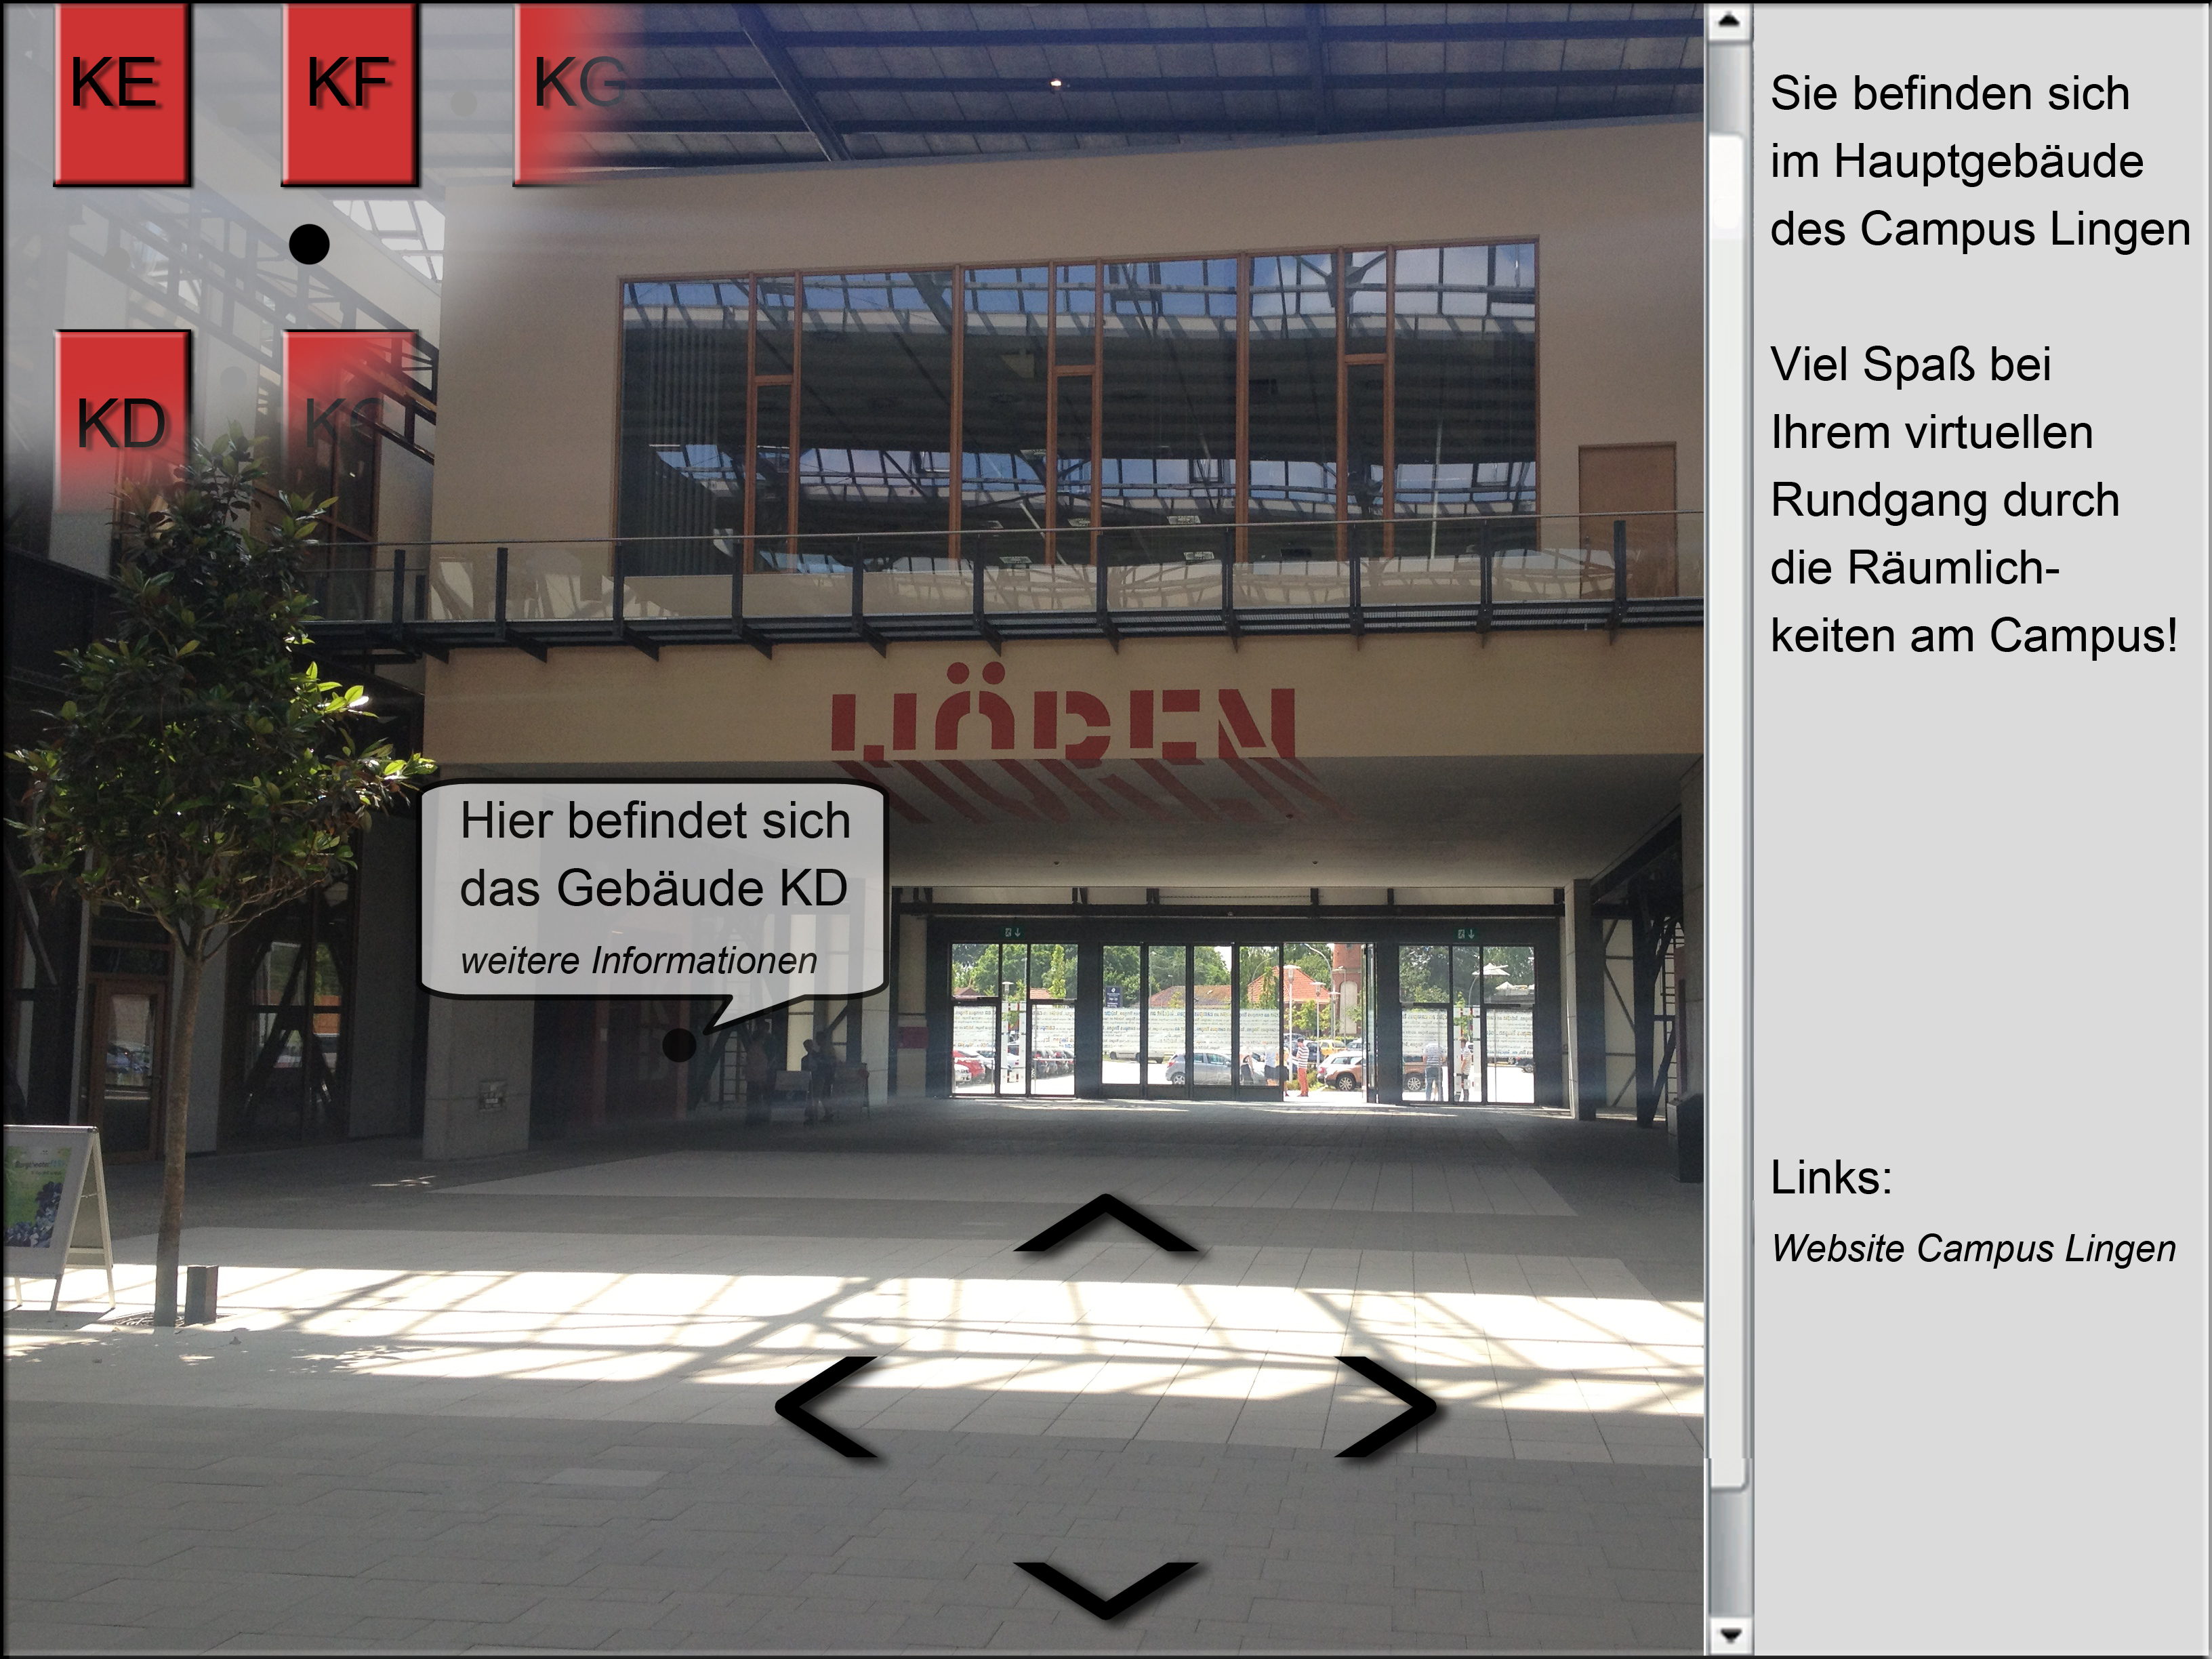
\includegraphics[width=1.0\textwidth]{MockupFrontend.jpg}
\caption[Mockup Benutzeransicht]{Oberflächenentwurf der
Benutzeransicht\protect\footnotemark}
\label{fig:MockupFrontend}
\end{figure}
\footnotetext{Quelle: Eigene Darstellung}

In diesem Mockup sind vier Elemente dargestellt, deren Funktion im Folgenden erläutert wird.

\begin{itemize}
 \item Ein 360-Grad Panorama
 \item Ein Steuerkreuz
 \item Eine kleine Übersichtskarte (Minimap)
 \item Ein Informationsfenster
\end{itemize}

Das \textbf{360-Grad Panorama} ist zentrales Element des Projektes. Dieses Panorama stellt einen Blickwinkel dar, von dem aus sich ein Benutzer den Campus Lingen ansehen kann. Von diesem Blickwinkel aus kann sich der Benutzer virtuell um die Vertikalachse der Fotoaufnahme drehen und dabei alles in diesem Blickwinkel betrachten. Er kann zudem die Aufnahme um 180-Grad horizontal drehen. Ein Benutzer hat damit von einen Standpunkt aus einen vollen Rundumblick.

Mit dem \textbf{Steuerkreuz} am unteren Rand des Panoramas kann ein Benutzer zu einem anderen Aufnahmepunkt wechseln. Er erhält damit einen Einblick aus einem anderen Blickwinkel und kann sich in diesem wiederum frei umsehen. Die Pfeile des Steuerkreuzes zeigen dabei zu jeder Panoramaaufnahme, die von der aktuellen Position erreichbar ist.

Die \textbf{Minimap} ist in einer der Ecken des Panoramas platziert und erfüllt zwei Aufgaben. Zum einen dient sie der Übersichtlichkeit und Orientierung des Benutzers. Sie zeigt an welcher Aufnahmeposition sich der Benutzer aktuell am Campus befindet (im Oberflächentwurf durch einen schwarzen Punkt gekennzeichnet). Hierdurch wird neben dem Einblick in die Räumlichkeiten des Campus auch ein Bild des Aufbaus vermittelt.
Zum anderen kann die Minimap, genau wie die Pfeile des Steuerkreuzes, zum Navigieren zu anderen Aufnahmen genutzt werden. Dazu werden alle Aufnahmepositionen, die sich im Sichtfeld des dargestellten Ausschnittes befinden, farblich hervorgehoben. Durch anklicken einer solchen Markierung wird der Benutzer in eine andere Aufnahmeposition versetzt. Beim wechseln der Aufnahmeposition verändert sich dabei auch der dargestellte Ausschnitt der Minimap.

Das \textbf{Informationsfenster} zeigt zu guter Letzt interessante Informationen zum aktuellen Panorama an. Im obigen Oberflächenentwurf sind zwei solcher Informationsfenster dargestellt (am rechten Rand und oberhalb des Steuerkreuzes). Diese Darstellungsformen sind als alternativ zu betrachten. Die Art der Informationsdarstellung ist zum Zeitpunkt des Öberflächenentwurfs noch nicht eindeutig festgelegt. Inhalt dieser Informationsfenster können dabei Interessante Projekte einzelner Studiengänge, Öffnungszeiten von Räumlichkeiten oder Wissenwertes aus dem Studienalltag sein. Die Anzeige der Informationsfenster ist dabei in einer Art Popup gedacht. Das heißt sie sollen nicht permanent angezeigt werden, sondern erscheinen erst durch Klick des Benutzers auf einen Button. Dadurch wird das Panorama und damit der Blick des Benutzers nicht durch störende Anzeigen eingeschränkt.
\subsubsection{Administrationsbereich}
\label{sec:UmsetzungAdministrationsbereich}

Der entwickelte Prototyp stellt eine erste lauffähige Version einer Benutzeransicht dar. Der nächste Entwicklungsschritt ist die Implementierung des Administrationsbereiche und die Bereitstellung von APIs. Aufbauend auf gepflegten Ìnformationen im Administrationsbereich wird der Prototyp dann um dynamische Funktionalität erweitert. Das heißt die angezeigten Panoramas und die benachbarten Panoramas werden über eine API angefragt, die die Informationen aus der Datenbank lädt. Der Implementierungsprozess des Administrationsbereiches wird dabei sukzessiv anhand der vorgestellten Anwendungsfällen (siehe \nameref{sec:Adminstratoranwendungen} auf Seite \pageref{sec:Adminstratoranwendungen}) realisiert. Prioresiert werden dabei die Anwendungsfälle, die die Verwaltung der Panoramas, Infotexte und die Übersichtskarte betreffen (AFA05 bis AFA17).

Bevor mit der Implementierung begonnen werden kann wird noch ein einheitliches Design festgelegt, dass vor allem dem späteren Administrator das Verständnis erleichtert. Zu diesem einheitlichen Design Konzept zählt zum Beispiel das Farbschema von Buttons. So wurde beispielsweise festgelegt, dass ein roter Button immer das Löschen eines Datensatzes signalisiert und ein grüner immer das speichern eines Datensatzes. Darüber hinaus wurde entschieden die Gestaltung von Buttons, Informationsfenster und ähnlichem mit dem CSS\footnotemark\ Framework Bootstrap\footnotemark\ zu realisieren. Dadurch ist gewährleistet, dass alle Steuerungselemente in allen Browsern gleich aussehen und der Administrator Elemente durch ihr Aussehen wiedererkennen und darüber auf ihre Benutzung schließen kann. Durch diese Entscheidungen wird die Usability der Software erhöht und der Aufwand der zu erstellenden Dokumentation verringert.

\footnotetext{CSS steht für Cascading Style Sheets und beschreibt eine Skriptsprache, die dazu dient HTML-Elemente in Form und Farbe zu verändern.}

\footnotetext{Bootstrap ist ein open Source Projekt, in dem einheitlich das Design von verschiedenen HTML-Elemente definiert ist. Bootstrap ist ein Projekt des Internetkonzerns Twitter und ist besonders dafür geeignet ein einheitliches Look and Feel einer Webseite in allen Browsern zu erzeugen.}

Aufbauend auf Administratoranwendungsfällen und Designkonzept werden Tickets erstellt, deren Inhalt die Implementierung der Infotext- und Fotoverwaltung ist. Zur Verdeutlichung der eingesetzten Technologien und des Entwicklunsablaufs wird im Folgenden eine stark vereinfachte Fotoverwaltungsseite implementiert. Implementiert werden soll eine Seite, die alle Fotos der Datenbank mit Namen und Beschreibung anzeigt. Zustätzlich soll es dem Administrator möglich sein auf den Namen eines Fotos zu klicken, woraufhin ihm weitere Informationen angezeigt werden.

Zur Implementierung dieses Szenarios wird zunächst ein HTML-Dokument angefertigt, dass das Grundgerüst der Fotoverwaltung darstellt. In diesem Grundgerüst könnten bestimmte Elemente, wie zum Beispiel die Navigationsbar am oberen Rand (vergleiche \abbildung{MockupBackend}) der Seite oder der Titel der Seite, statisch codiert werden. Zur Vereinfachung soll aber nur der Titel der Seite gesetzt werden und eine Überschrift. Das folgende \listing{HTML_Anwendungsbeispiel} zeigt das angefertigte HTML-Dokument.

\lstinputlisting[language=HTML,caption={statisches HTML},label={lst:HTML_Anwendungsbeispiel}]{Listings/HTML_Anwendungsbeispiel.html}

Im Anschluss daran muss die Seite um dynamisch generierten Inhalt erweitert werden. Dynamischer Inhalt ist im gegeben Anwendungsfall das Anzeigen aller Fotos, die bereits in der Datenbank sind. Um dieses Verhalten zu realisieren muss eine Anfrage an die Datenbank gestellt werden und danach muss für jeden Eintrag in der Datenbank HTML Quellcode geschrieben werden. Das nachfolgende \listing{HTML mit PHP} zeigt die Implementierung mit PHP.

\lstinputlisting[language=HTML,caption={Dynamisches schreiben von HTML mit PHP},label={lst:HTML mit PHP}]{Listings/HTML_mit_PHP.php}

Zu sehen ist die Anfrage an die Datenbank, die durch die PHP-Funktion "`mysql\_query"' (Zeile 5) realisiert wird, das Durchlaufen jeden Datenbanksatzes in einer Schleife (Zeile 6ff.) und das schreiben von HTML mit dem PHP "`echo"'-Befehl.

Zum Abschluss wird das klicken auf den Fotonamen implementiert. Diese Benutzerinteraktion kann am besten auf dem Clientsystem des Benutzers (Internetbrowser) mit Javascript verarbeitet werden, da keine weiteren Informationen vom Server benötigt werden und zusätzliche Anfragen so vermieden werden. Javascript-Routinen werden meistens als Funktionen formuliert, die aufgerufen werden, wenn ein bestimmtes Ereignis eintritt. Im \listing{HTML mit PHP} ist ein solcher Funktionsaufruf in Zeile 9 zu sehen. Die Funktion "`toggleDescription"' wird aufgerufen sobald auf das <p>-Tag geklickt wird. Als Parameter wird dieser Funktion das eigene HTML-Element, also das <p>-Tag, mitgegeben. Die Javascript-Funktion ist in \listing{Javascript Snippet} dargestellt.

\lstinputlisting[language=JavaScript,caption={Auf Benutzerinteraktion reagieren mit Javascript},label={lst:Javascript Snippet}]{Listings/Javascript_Snippet.js}

Alle dargestellten Listings könnten dabei in einem Dokument stehen, das vom dem Administrator über seinen Internetbrowser angefragt wird.
Wie bereits erwähnt ist diese Darstellung der Implementierung sehr stark vereinfacht. Die Quelldateien, die die Fotoverwaltung im vorliegenden Projekt implementieren, sind zu umfangreich, um sie an dieser Stelle zu präsentieren. Die implementierte Fotoverwaltung wird in folgendem Bildschirmfoto zur Veranschaulichung dargestellt:

%TODO: Bildschirmfoto ohne Pixelfehler machen.
\begin{figure}[htb]
\centering
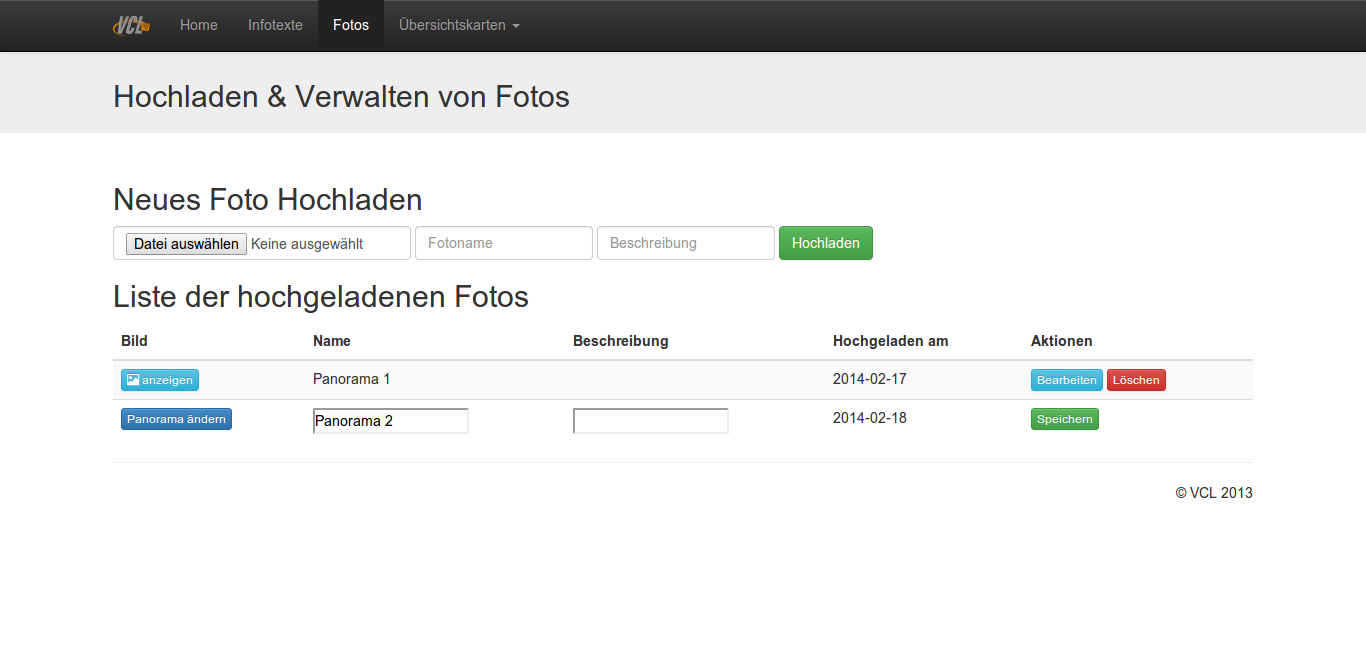
\includegraphics[width=1.0\textwidth]{Fotoverwaltung.png}
\caption[Fotoverwaltung]{Bildschirmfoto der implementierten Fotoverwaltung}
\label{fig:Fotoverwaltung}
\end{figure}

In einem solchen Entwicklungszyklus wurde auch die Verwaltung der Infotexte und die Übersichtskarte implementiert. Bildschirmfotos dieser Bereiche sind im Anhang dargstellt, siehe \abbildung{ScreenshotInfotext}, \abbildung{ScreenshotUebersichtskarte}.
\subsection{Anwendungsfälle}
\label{sec:Anwendungsfaelle}

% TODO: Anhang der use case diagramme verweisen

Aufbauend auf dem Entwurf der Oberfläche sowohl für den Benutzer, als auch für den Administrator, werden im Folgenden Anwendungsfälle beschrieben, die die Anwendungsmöglichkeiten dieser beiden Benutzergruppen beschreiben. Zur visuellen Modellierung dieser Anwendungsfälle wird die Darstellungsart des Anwendungsfalldiagramms (use case diagram)\footnotemark gewählt. Die Diagramme sind im Anhang dargestellt.

\footnotetext{Ein Anwendungsfalldiagramm ist eine Diagrammart der Unified Modelnig Langauge, kurz UML. In dieser werden sowohl Auslöser einer Funktion als auch Funktionsbeschreibung dargestellt. Eine Funktion kann dabei weitere Funktionen einbinden oder erweitern.}

Die im Folgenden vorgestellten Anwendungsfälle dienen sowohl der Dokumentation der Anwendungs, als auch zur späteren Durchführung der Tests.
\subsubsection{Benutzeranwendungen}
\label{sec:Benutzeranwendungen}

Ein Benutzer der Software hat verschiedene Möglichkeiten der Interaktion mit
der Anwendung. Diese sind im Folgenden mit der fortlaufenden
Kennzeichnung \textbf{AFBXX}\footnote{AFBXX = Anwendunsfall eines Benutzers mit
Nr. XX} markiert und strukturiert aufgelistet:

\begin{description}
  \item[AFB01] Der Benutzer ruft die Webanwendung durch einen Internetbrowser
  auf.
  \item[AFB02] Der Benutzer dreht sich horizontal und vertikal um die Achse
  der Fotoaufnahme, um einen Rundumblick zu erhalten.
  \item[AFB03] Der Benutzer zoomt über die Steuerelemente in die Fotoaufnahme
  hinein.
  \item[AFB04] Der Benutzer navigiert mit Hilfe der Navigationselemente zu
  anderen Aufnahmepositionen.
  \item[AFB05] Der Benutzer navigiert mit Hilfe der Minimap zu einer anderen
  Aufnahmeposition.
  \item[AFB06] Der Benutzer bewegt sich mit Hilfe der Pfeiltasten seiner
  Tastatur zu anderen Aufnahmepositionen
  \item[AFB07] Der Benutzer öffnet über ein Steuerungselement ein
  Informationsfenster.
  \item[AFB08] Der Benutzer schließt über ein Steuerungselement ein
  Informationsfenster.
\end{description}

% TODO: Verweise auf Anwenwendungsfalldiagram, Anhang, und Seite korrekt einfügen
Die Anwendungsfälle AFB01 bis AFB08 definieren die Menge an
Interaktionsmöglichkeiten eines Benutzers. Diese Menge an
Interaktionsmöglichkeiten ist inklusive der hinterlegten Funktionen im
Awendungsfalldiagramm im \anhang{BenutzerAnwendungsfalldiagramme} abgebildet.

\subsubsection{Adminstratoranwendungen}
\label{sec:Adminstratoranwendungen}

Ein Administrator hat in vier Bereichen Möglichkeiten zur
Steuerung und Pflege der Webanwendung. Diese vier Bereiche wurden im
\verweis{Administrationsbereich} vorgestellt. Die Möglichkeiten der Interaktion
in diesen Bereichen sind mit der forlaufenden
Kennzeichnung \textbf{AFAXX}\footnote{AFAXX = Anwendunsfall eines Adminstrator
mit Nr. XX} markiert und strukturiert aufgelistet:

\begin{description}
  \item[AFA01] Der Adminstrator ruft den Administrationsbereich der
  Webanwendung durch einen Internetbrowser auf.
  \item[AFA02] Der Administrator klickt auf den Menüpunkt "`Infotexte"' und ihm
  wird die Infotextverwaltung angezeigt.
  \item[AFA03] Der Administrator erstellt im Menüpunkt "`Infotexte"' einen neuen
  Informationstext.
  \item[AFA04] Der Administrator verändert im Menüpunkt "`Infotexte"' einen
  erstellten Informationstext.
  \item[AFA05] Der Administrator löscht im Menüpunkt "`Infotexte"' einen
  erstellten Informationstext.
  \item[AFA06] Der Administrator klickt auf den Menüpunkt "`Fotos"' und ihm wird
  die Fotoverwaltung angezeigt.
  \item[AFA07] Der Administrator lädt im Menüpunkt "`Fotos"' ein erstelltes
  Panoramafoto mit Beschreibung und Namen hoch.
  \item[AFA08] Der Administrator verändert im Menüpunkt "`Fotos"' den Namen und
  die Beschreibung eines hochgeladenen Fotos.
  \item[AFA09] Der Administrator löscht im Menüpunkt "`Fotos"' ein hochgeladenes
  Foto.
  \item[AFA10] Der Administrator klickt auf den Menüpunkt "`interssante Orte"'
  und ihm wird die Verwaltung der interessanten Orte angezeigt.
  \item[AFA11] Der Administrator erstellt im Menüpunkt "`interssante Orte"'
  einen neuen interessanten Ort.
  \item[AFA12] Der Administrator verändert im Menüpunkt "`interssante Orte"' den
  Namen und die Beschreibung zu einem interessanten Ort.
  \item[AFA13] Der Administrator löscht im Menüpunkt "`interssante Orte"' einen
  interessanten Ort.
  \item[AFA14] Der Administrator klickt auf den Menüpunkt "`Übersichtskarte"'
  und ihm wird die Übersichtskarte angezeigt.
  \item[AFA15] Der Administrator platziert im Menüpunkt "`Übersichtskarte"' ein
  hochgeladenes Foto auf der Übersichtskarte.
  \item[AFA16] Der Administrator verschiebt im Menüpunkt "`Übersichtskarte"' ein
  bereits platziertes Foto an eine andere Position.
  \item[AFA17] Der Administrator navigiert im Menüpunkt "`Übersichtskarte"' über
  die Steuerelemente zu einem anderen Stockwerk.
  \item[AFA18] Der Administrator verbindet im Menüpunkt "`Übersichtskarte"'
  mehrere hochgeladene und positionierte Fotos auf der Übersichtskarte.
  \item[AFA19] Der Administrator verbindet im Menüpunkt "`Übersichtskarte"' ein
  hochgeladenes und positioniertes Foto mit erstellten Informationstexten.
\end{description}

% TODO: Verweise auf Anwenwendungsfalldiagram, Anhang, und Seite korrekt einfügen
Die Anwendungsfälle AFA01 bis AFA19 definieren die Menge an
Interaktionsmöglichkeiten eines Administrators. Diese Menge an
Interaktionsmöglichkeiten ist inklusive der hinterlegten Funktionen in einem
Awendungsfalldiagramm im Anhang X auf Seite X dargestellt.

\subsection{Datenbankentwurf}
\label{sec:Datenbankentwurf}

Aufbauend auf den vorangegangenen Entwurfsergebnissen wird im Folgenden ein
Entwurf der Datenbank in Form eines Tabellenmodells angefertigt.\footnote{Ein
Tabellenmodell ist ein graphisches Modell zur Darstellung der Struktur einer
Datenbank. In diesem Modell werden Tabellen, deren Attribute (Eigenschaften)
und die Beziehung zu anderen Tabellen dargestellt.}

Bevor das Tabellenmodell erstellt werden kann, müssen in dem vorliegenden
Projekt die Daten identifiziert werden, die persistent in der Datenbank
gespeichert werden. Aus dem vorgangenen Oberflächenentwurf wird deutlich, dass
das Projekt aus den zwei Teilen, Benutzeransicht und Administrationsansicht,
besteht. Die Benutzeransicht stellt dabei Informationen dar, die in der
Administrationsansicht gepflegt und hinterlegt wurden. Der
Administrationsbereich ist der datenhaltende Bereich, in dem die Interaktion
mit der Datenbank stattfindet. Aus dem \verweis{Administrationsbereich} ergeben
sich bereits folgende drei Informationsobjekte:

\begin{itemize}
  \item Infotexte
  \item Fotos
  \item Interessante Orte
\end{itemize}

Die Beziehung zwischen Infotexten und Fotos stellt dabei eine sogenannte
n:m Beziehung dar. In dieser Beziehung kann ein Infotext mehreren Fotos
zugeordnet sein und im Gegenzug können ebenso mehrere Infotexte auf demselben
Foto platziert werden. Um eine soche Beziehung in einer relationalen Datenbank
abbilden zu können muss eine neue Tabelle angelegt werden, die diese Beziehung
zwischen Foto und Infotext speichert. Gleiches gilt für die
Nachbarschaftsbeziehung zwischen zwei Fotos. Da ein Foto mehrere Nachbarfotos
haben kann muss wiederum eine Tabelle erstellt werden, in der die Beziehung
zwischen Foto und Nachbarfoto gespeichert wird. Neben diesen zwei zusätzlichen
Tabellen werden noch drei weitere Tabellen für die Speicherung der Daten der
Übersichtskarte benötigt. In der Übersichtskarte soll grundsätzlich zwischen dem
Studienstandort an der Baccumer Straße und dem Standort an der Kaiserstraße
unterschieden werden. Da beide Standorte unterschiedlich parametresiert werden 
müssen wird hierfür eine eigene Tabelle benötigt. Diese wird mit dem Namen
\textit{Area} bezeichnet. Eine Area beschreibt hierbei einen topologischen
Auschnitt einer Google Maps Karte. Da eine topologische Karte nur den Umriss von
Gebäuden zeigt, ist es schwer, den genauen Standort eines Panoramas zu
bestimmen. Aus diesem Grund werden Grafiken über die Karte gelegt, die die
innere Struktur (Wände, Gebäudetrackte, etc.) des Campus zeigen. Sowohl die
topologische Karte als auch die übergelegten Grafiken, im folgenden
\textit{Overlays} genannt, benötigen eine eigene Tabelle, da beide jeweils noch
weitere Attribute haben. Ein Overlay ist dabei immer einer Karte zugeordnet.
Eine Karte kann weiterhin mehrere Overlays besitzen. Über die Zuordnung von
mehreren Overlays zu einer Karte werden Stockwerke an einem Standort
dargestellt. Ein Overlay enthält damit unter anderem den Pfad zu einer Grafik,
die ein Stockwerk an einem Standort darstellt. Zusamengefasst ergeben sich
folgende Tabellen:

\begin{itemize}
  \item infotext (Verwaltung der Infotexte)
  \item panorama (Verwaltung der Fotos)
  \item poi (Verwaltung der interessanten Orte)
  \item infotext\_panorama (n:m-Beziehung zwischen Infotexten und Fotos)
  \item neighbour (n:m-Beziehung zwischen zwei Fotos)
  \item area (Kartenbereich)
  \item map (Kartenansicht)
  \item overlay (übergelegte Grafik)
\end{itemize}

Diese Tabellen werden in \abbildung{Tabellenmodell} mit ihren jeweiligen
Attributen und Beziehungen dargestellt.

\begin{figure}[htb]
\centering
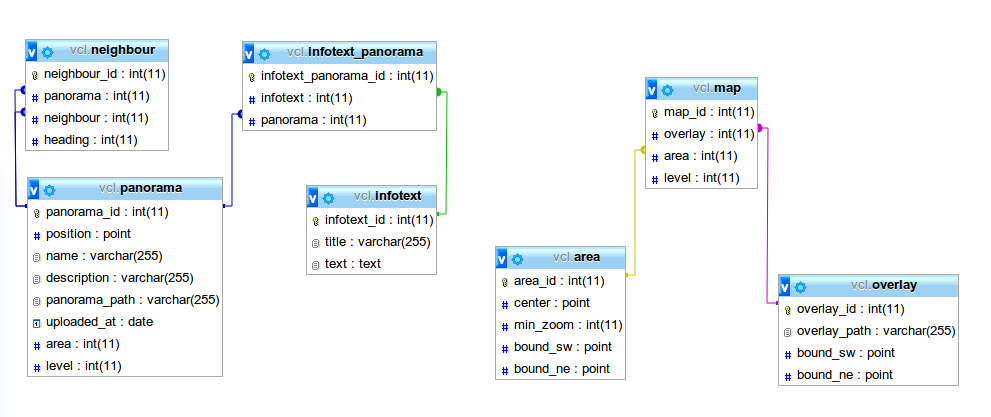
\includegraphics[width=1.0\textwidth]{Tabellenmodell.png}
\caption[Tabellenmodell der Anwendung]{Tabellenmodell der Anwendung\protect\footnotemark}
\label{fig:Tabellenmodell}
\end{figure}
\footnotetext{Quelle: Eigene Darstellung}
\subsection{Architektur}
\label{sec:Architektur}

Der Architekturentwurf des vorliegenden Projektes wurde bereits im \verweis{Architekturgrundlagen} als Ausgangsbasis zur Erläuterung der Grundlagen präsentiert. Aufbauend auf diesen Grundlagen wird der Architekturentwurf im Folgenden genauer betrachtet. Ausgangspunkt der folgende Darstellung ist die Architektur, die in \abbildung{Architektur} zu sehen ist.

\begin{figure}[htb]
\centering
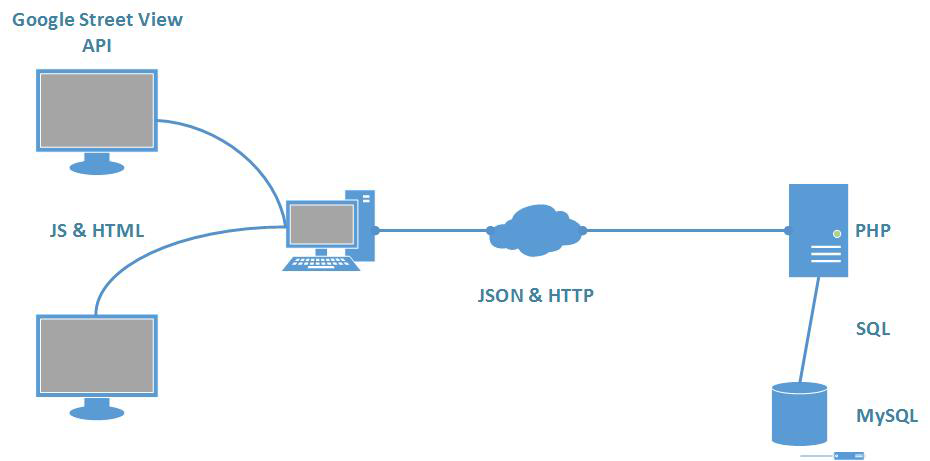
\includegraphics[width=1.0\textwidth]{Architektur.png}
\caption[Architektur der Anwendung]{Architektur der
Anwendung\protect\footnotemark}
\label{fig:Architektur}
\end{figure}
\footnotetext{Quelle: Eigene Darstellung}

Der dargestellte Architekturentwurf zeigt eine klassische Client-Server-Architektur. Das bedeutet die Architektur lässt sich in zwei Subsysteme aufteilen, die über definierte Schnittstellen kommunizieren können. Diese Kommunikation besteht immer in Form von Anfrage und Antwort. Ein Subsystem fragt dabei einen Dienst an, den das andere Subsystem anbietet. Das Clientsubsystem ist dabei definiert als das Subsystem, dass einen Dienst des Serversubsystems anfragt. Das Serversubsystem bietet damit einen Dienst an\footnote{\citet[S.~177]{rautenstrauch2002}}.

Im vorliegenden Projekt stellt das Serversystem vor allem Webdokumente und Schnittstellen (APIs) für das Clientsystem bereit. Zur Realisierung dieser Schnittstellen wird die Serverskriptsprache PHP und eine MySql-Datenbank eingesetzt. Bei der Anfrage eines Webdoukemnts wird auf dem Serversystem eine PHP-Routine durchgeführt und als Antwort ein HTML Dokument zurückgeliefert. Inhalt der PHP-Routine kann dabei eine Anfrage an die Datenbank sein, auf der aufbauend HTML dynamisch generiert wird.
Bei Anfragen an sogenannte Application Programming Interfaces (APIs) werden ebenfalls Informationen mit Hilfe von PHP aus der Datenbank gelesen und in einem definierten Format zurückgeliefert. Im Gegensatz zu Webdokumenten ist eine solche Schnittstelle (engl: interface) für den Informationsaustausch zwischen Programmen ausgelegt ist. Das Ausgabeformat der dargestellten Informationen ist aus diesem Grund nicht für menschliche Lesbarkeit optimiert.

Die Anfragen an den Server werden durch den Benutzer initiert und die zurückgelieferten Antworten werden interpretiert. Das Clientsystem ist dabei im vorliegenden Projekt der Internetbrowser eines Benutzers. Dieser löst durch das Aufrufen von Webseiten anfragen aus, der Server beantwortet diese und der Internetbrowser des Benutzers stellt das zurückgelieferte HTML dar. Eine solche Anfrage ist ein Anwendungsbeispiel für eine Anfrage nach einem Webdoukment. Darüber hinaus werden auf dem Client Routinen der Programmiersprache Javascript ausgeführt.
Durch Javascript können dabei Benutzerinteraktionen direkt auf dem Client verarbeiten werden. Das steigert die Performanz, da keine erneuten Anfragen an den Server geschickt werden müssen. Über diese Technologie ist auch die Google Street View API eingebunden. Diese erlaubt es 360-Grad-Fotos darzustellen und zu weiteren festgelegten Panoramas zu navigieren.
\subsection{Pflichtenheft}
\label{sec:Pflichtenheft}

% TODO: Auf einzelne Punkte des Pflichtenheftes eingehen oder nicht?
Aufbauend auf Datenbankentwurf und Archtiekturdesign wird die Entwurfsphase mit der Erstellung eines Pflichtenheftes abgeschlossen. Die Spezifikationen des Lastenheftes werden darin aus Entwicklersicht konkretisiert. Zum Verständnis des vorliegenden Projektes reichen aber die Angaben des Lastenheftes (siehe Seite \pageref{sec:Lastenheft}). Das Pflichtenheft wird aus diesem Grund an dieser Stelle nicht explizit angeführt. Es kann aber in \citet{pflichtenheft2013} nachgelesen werden.
\section{Umsetzung}
\label{sec:Umsetzung}
\subsection{Panoramaerstellung}
\label{sec:Panoramaerstellung}

\subsubsection{Anforderungen an die Panoramafotos}
\label{sec:PanoramaerstellungAnforderungen}

Die Panoramaerstellung stellt, neben der Softwareerstellung einen zentralen
Teilprozess innerhalb der Projektumsetzung dar. Bevor mit der Erstellung der
Panoramas begonnen werden kann müssen zunächst die Anforderungen der Anwendung
an die Panoramafotos festgelegt werden. Hierbei muss definiert werden, welche
Kriterien die Panoramafotos erfüllen müssen, um von der Anwendung korrekt
verarbeitet werden zu können. Relevante Kriterien sind hierbei die
Darstellungsform, die Größe und das Format der Panoramafotos. Nachdem diese
Schnittstelle festgelegt ist kann der Prozess der Panoramaerstellung isoliert
vom Prozess der Softwareerstellung durchgeführt werden. Dies ermöglicht eine
parallele Umsetzung der beiden Teilprozesse.

Wie bereits in \verweis{Architektur} erwähnt soll in der Anwendung die Google
Street View API verwendet werden. Diese Schnittstelle stellt die Funktionalität
zur Anzeige der Panoramafotos zur Verfügung. Somit legt diese Schnittstelle auch
fest, in welcher Form die Panoramafotos zur Verfügung gestellt werden müssen.
Diese Anforderungen können aus der Entwicklerdokumentation zu der API entnommen
werden. Die Schnittstelle erwartet hierbei ein Panoramafoto, welches der
Rektangulatprojektion\footnote{Die Rektangularprojektion stellt eine
horizontale Ansicht von 360 Grad und eine vertikale Ansicht von 180 Grad dar.
Dies bedingt ein Seitenverhälnis von 2:1} entspricht. Durch die API wird diese
Darstellung auf die Fläche einer Kugel projeziert. Der Mittlepunkt dieser Kugel
stellt den Standpunkt des Betrachters dar. Da sich immer nur ein Teil der
Projektion im Blickfeld dieses Betrachters befindet muss auch nur der aktuell
sichtbare Bereich des Panoramafotos dargestellt werden. Aus diesem Grund bietet
die Google Street View API die Möglichkeit, ein in mehrere rechteckige Teile,
sogenannte Kacheln, aufgeteiltes Panoramafoto zu verarbeiten. Auf diese Weise
kann die Performanz der Anwendung erhöht werden, da nicht das komplette
Panoramafoto, sondern nur ein Teil der Kacheln in der Anwendung geladen werden
muss. Damit den einzelnen Kacheln die korrekte Position auf der Planarprojektion
zugewiesen werden kann, muss die Benennung der Kacheldateien dem Namensschema
\texttt{Kachelspalte-Kachelzeile} genügen. Die Anzahl der Kacheln sowie die
Pixelmaße des Panoramafotos können frei gewählt werden. Hierbei ist zu beachten,
dass mit steigender Pixelanzahl die Qualität der 360-Grad-Darstellung steigt,
die Performance der Anwendung jedoch aufgrund der steigenden Datengröße sinkt.
In einer prototypischen Implementierung, auf die im \verweis{Softwareerstellung}
näher eingegangen werden soll, hat die Projektgruppe verschiedene Kombinationen
aus Pixekmaße und Kachelanzahl getestet. Letztendlich hat sich die Projektgruppe
auf die Pixelmaße 4096x2048 für das gesamte Panorama und eine Aufteilung in 32
Kacheln entschieden. Diese Kombination wurde einheitlich als bester Kompromiss
zwischen Qualität und Performanz angesehen.
\subsubsection{Workflow der Panoramaerstellung}
\label{sec:Workflow}

Der Workflow der Panoramaerstellung kann in mehrere Teilprozesse untergliedert
werden. Für die Umsetzung dieser einzelnen Teilschritte wird hierbei spezielles
Hard- und Softwareequipment benötigt. Im Folgenden sollen die einzelnen
Teilschritte der Panoramaerstellung in chronologischer Reihenfolge erläutert
werden. Im Zuge dessen soll auch auf das benötigte Equipment eingegangen
werden.

\paragraph{Aufnahme der Einzelfotos} \hfill \\

Die Panoramaerstellung beginnt mit der Aufnahme mehrerer Einzelfotos. Aus diesen
Einzelfotos wird nachfolgend dann das komplette Panoramafoto zusammengefügt.
Dieses muss, wie zuvor erläutert, der Rektangularprojektion entsprechen. Die
Summe der Einzelfotos muss also eine horizontale Ansicht von 360 Grad und eine
vertikale Ansicht von 180 Grad abbilden. Die Anzahl der Einzelfotos ist somit
von dem Bildwinkel abhängig, der auf einem einzelnen Foto dargestellt werden
kann. Dieser Bildwinkel wird in der Fotografie durch die Brennweite des
Objektives festgelegt. Je geringer die Brennweite eines Objektives ist, desto
größer ist der Bildwinkel, der mit diesem Objektiv eingefangen werden kann und
desto weniger Einzelfotos werden für die Erstellung eines Panoramafotos
benötigt. Durch spezielle Objektivkonstruktionen wie zum Beispiel einem
Fisheye-Obektiv ist es möglich einen besonders großen Bildwinkel aufzunehmen.
Ein solches Objektiv und eine zum dem Objektiv kompatible Kamera wird auch für die Aufnahme der
Panoramafotos im Projekt verwendet. Das Objektiv ermöglicht es in 16 Fotos alle
Ansichten Aufzunehmen, die zur Darstellung einer Rektangularprojektion benötigt
werden. In 15 dieser Einzelfotos ist hierbei die horizontale Rundumansicht
dargestellt. Das sechzehnte Foto bildet den Zenit\footnote{Der Zenit ist der
Punkt über dem Beobachter/der Kamera} im Panoramafoto ab. Der
Nadir\footnote{Der Nadir ist der dem Zenit gegenüber gelegene Punkt unter dem
Beobachter/der Kamera} wird in den Panoramafotos nicht abgebildet, da sich hier
das Stativ befindet.

Zur Unterstützung bei der Aufnahme hat sich die Projektgruppe weiterhin
entschieden ein speziell für die Panoramafotografie ausgelegtes Stativ zu
verwenden. Eine Aufnahme ohne dieses Stativ wäre zwar denkbar, würde die
Qualität der Panoramafotos jedoch stark beeinträchtigen. Das Panoramastativ
besteht aus folgenden Komponenten:

\begin{description}
\item[Stativ] Das eigentliche Stativ dient dazu, die Kamera im Raum an einer
festen Position zu fixieren. Hierdurch ist sichergestellt, dass alle
Einzelfotos von der selben Position aus aufgenommen werden.
\item[Nivelliervorrichtung] Die Nivelliervorrichtung dient dazu, den Kopf des
Statives horitontal auszurichten. Auf diese Weise wird ein wellenförmiger
Horizont in dem zusammengefügten Panoramafoto vermieden.
\item[Rotator] Der Rotator ermöglicht es, den Kopf des Stativs um die vertikale
Achse zu drehen. Weiterhin kann eine Gradzahl festgelegt werden, nachdem der
Mechanismus bei einer Drehnung einrastet. Auf diese Weise wird eine gleichmäßige
Drehung bei der Aufnahme der Panoramafotos ermöglicht.
\item[Nodalpunktadapter] Der Nodalpunktadapter ermöglicht es, die Kamera auf
dem Stativ so zu positionieren, dass die Eintrittspupille des Stativs auf Höhe
der vertikalen Drehachse des Stativs liegt. Hierdurch können
Parallaxenfehler\footnote{Der Parallaxenfehler beschreibt eine scheinbare
Verschiebung zweier hintereinandergelegener Gegenstände, wenn sich der
Ausgangspunkt der Betrachtung ändert} bei der Aufnahme vermieden werden
\end{description}

Das komplette Equipment, welches zur Aufnahme der Panoramafotos verwendet wurde,
ist in \abbildung{Equipment} dargestellt.

\begin{figure}[htb]
\centering
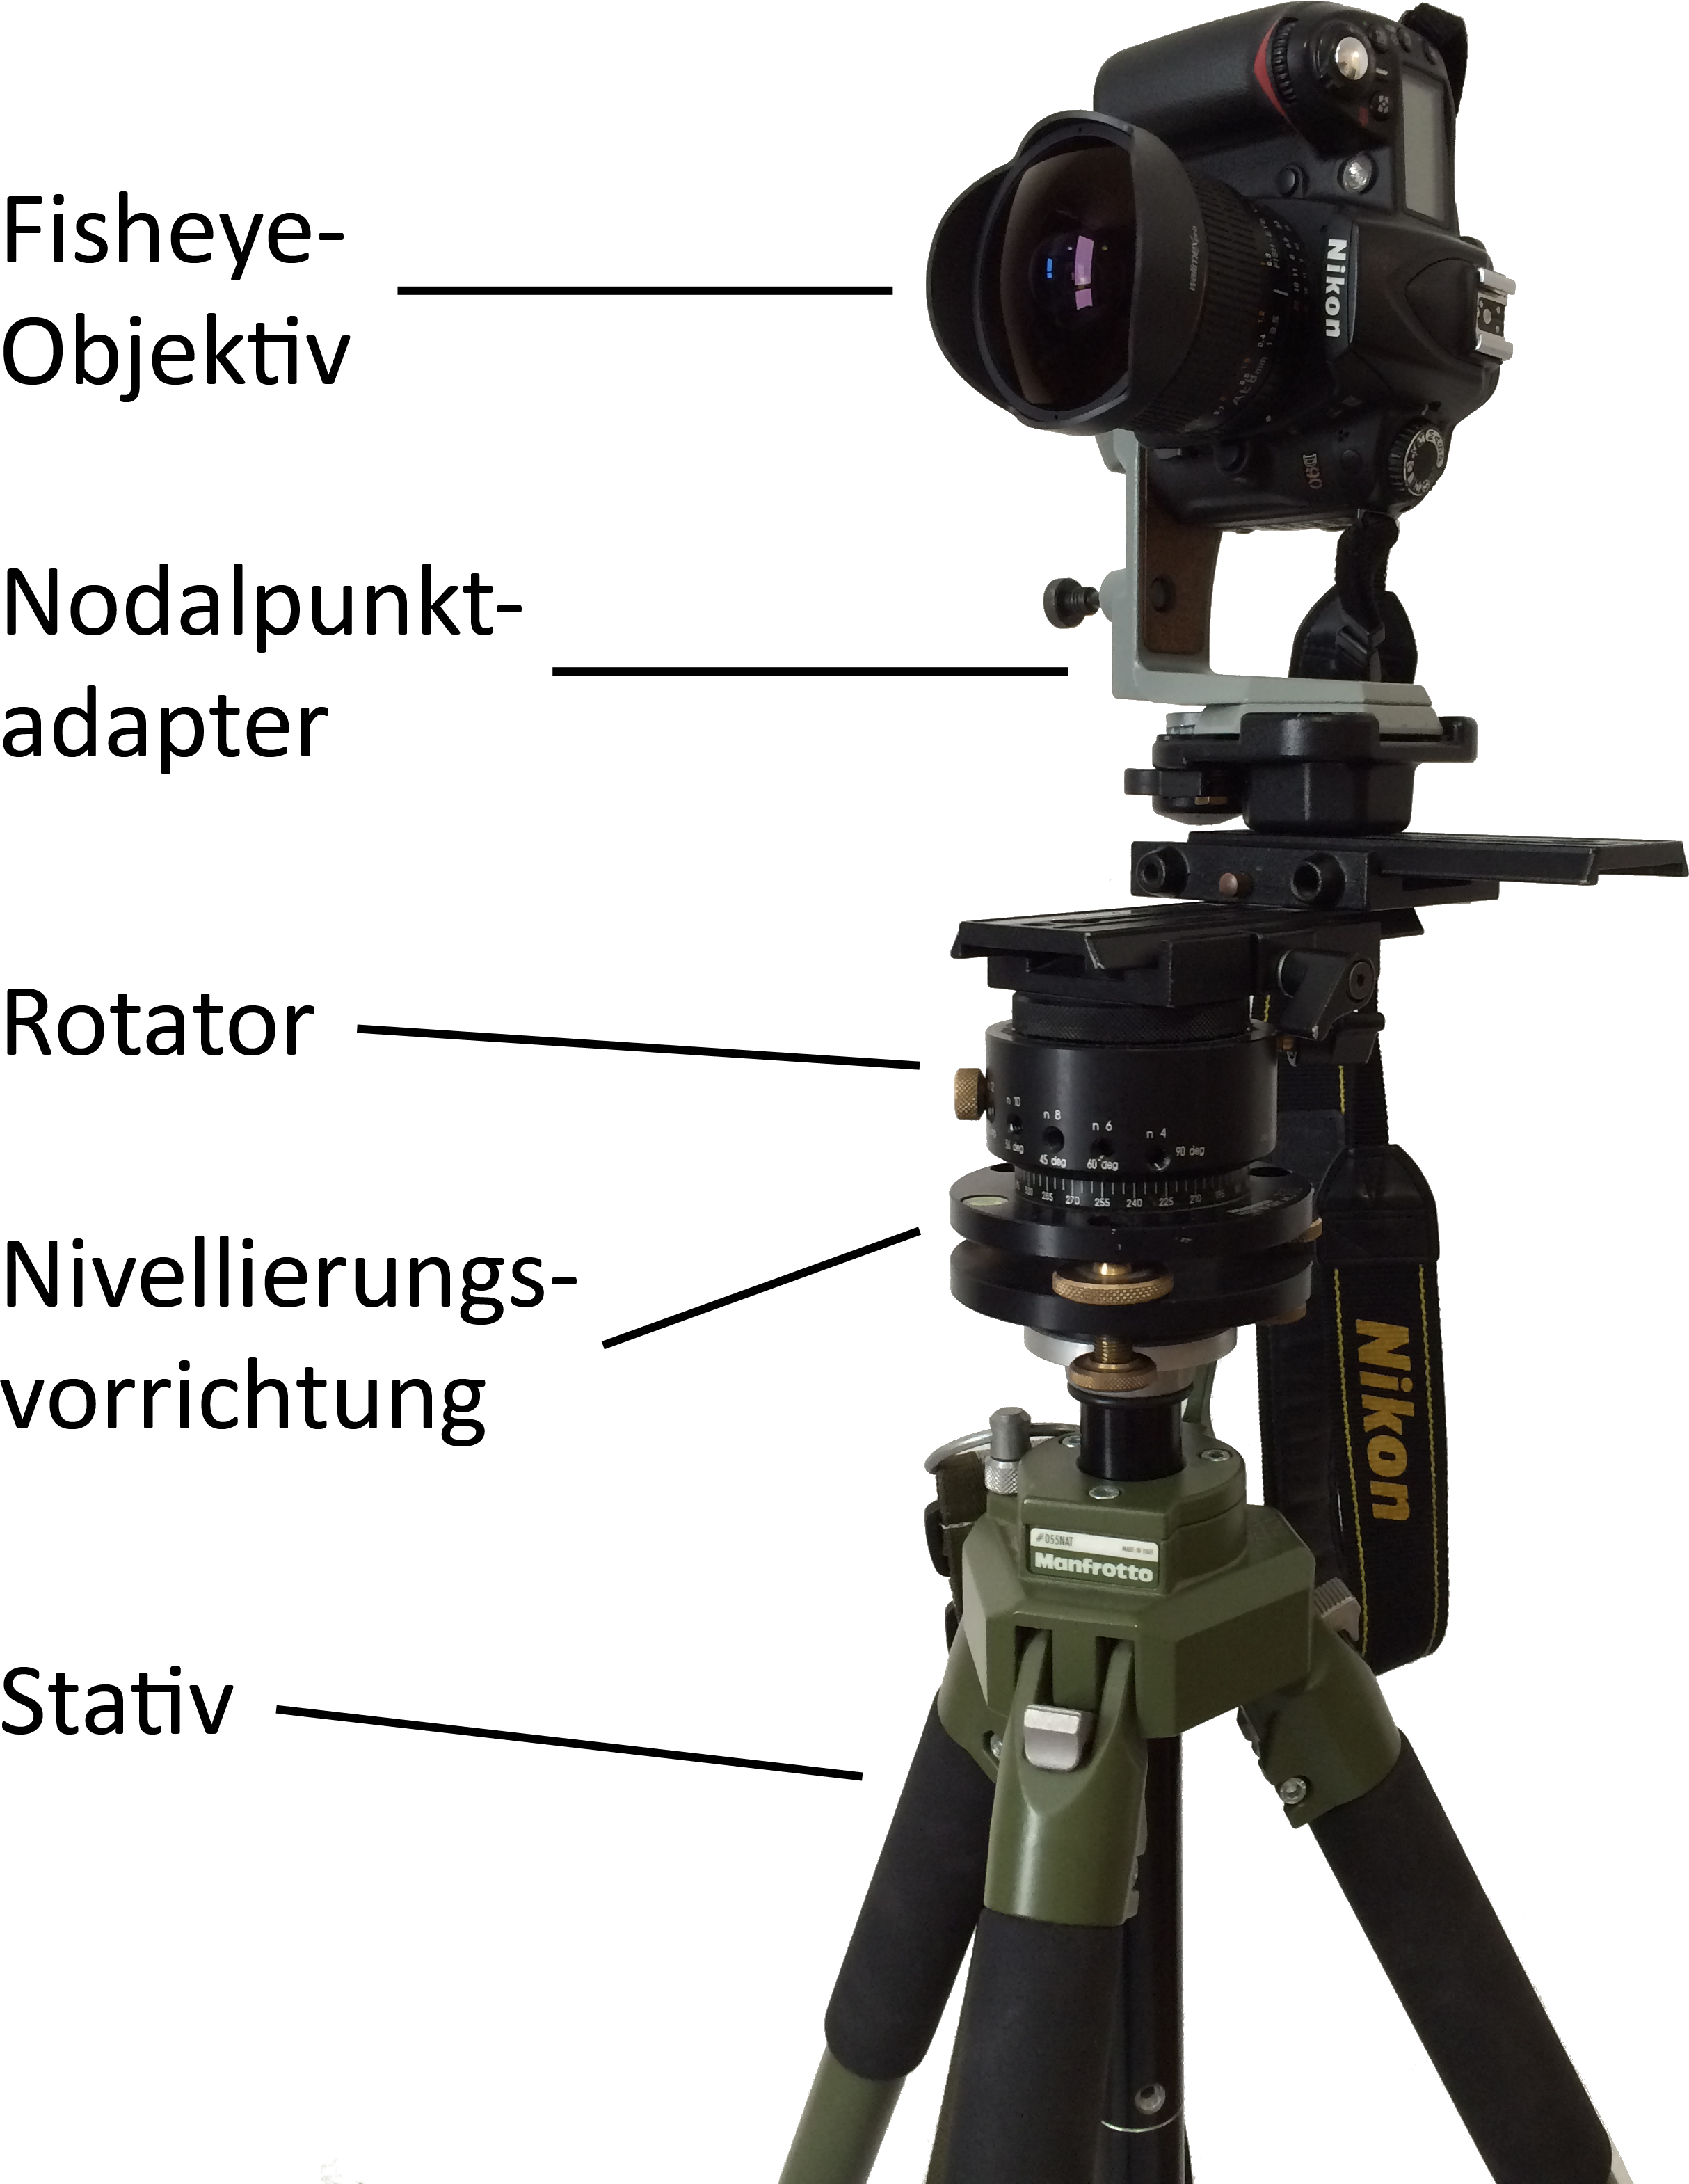
\includegraphics[width=0.5\textwidth]{Equipment.png}
\caption[Equipment zur Aufnahme der Einzelfotos]{Equipment zur Aufnahme der Einzelfotos\protect\footnotemark}
\label{fig:Equipment}
\end{figure}
\footnotetext{Eigene Darstellung}

\clearpage

\paragraph{Stitching und Rendering} \hfill \\

Nachdem die Einzelfotos aufgenommen wurden müssen diese zu einem Panoramafoto
zusammengefügt werden. Dieser Prozess wird als Stitching bezeichnet. Das
Stitching erfolgt im Projekt mit der Software Kolor Autopano Giga 3.0. Die
Software ist in der Lage, die Einzelfotos automatisiert zusammenzufügen.
Gegebenenfall muss das hieraus resultierende Panoramafoto nach dem
automatisierten Zusammenfügen noch manuell ausgerichtet werden. Aufgrund
dieser manuellen Ausrichtung ist es nicht möglich, den hier beschriebenen
Prozess vollständig zu automatisieren. In einem letzen Schritt wird das
zusammengefügte Panoramafoto dann in das JPEG-Format konvertiert. Dieser Schritt
wird als Rendering bezeichnet. Das Ergebnis dieses Prozesses ist in
\abbildung{Zusammengefuegt} dargestellt.

\begin{figure}[htb]
\centering
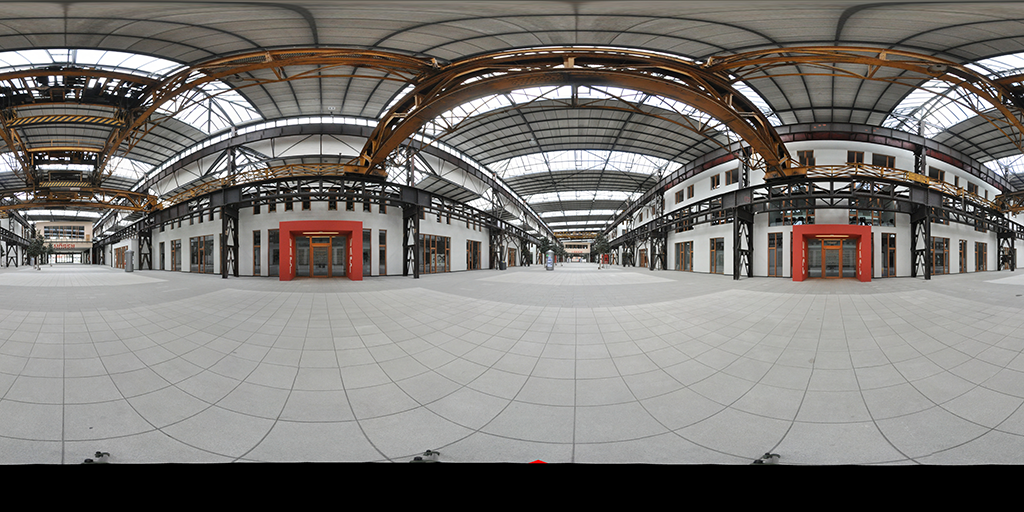
\includegraphics[width=0.8\textwidth]{Zusammengefuegt.png}
\caption[Panoramafoto nach Stitching und Rendering]{Panoramafoto nach Stitching
und Rendering\protect\footnotemark}
\label{fig:Zusammengefuegt}
\end{figure}
\footnotetext{Eigene Darstellung}

\paragraph{Überarbeitung und Optimierung der Panoramafotos} \hfill \\

Da es bei der Aufnahme der Einzelfotos nicht möglich war den Nadir abzubilden,
fehlen diese Informationen folglich auch in dem zusammengefügten
Pa\-no\-ra\-ma\-fo\-to. In \abbildung{Zusammengefuegt} ist der Bereich, in dem
die Bildinformationen fehlen, durch eine schwarze Fläche markiert. Im Zuge
einer Überarbeitung der Panoramafotos soll dieser schwarze Bereich mit einem
Label überdeckt werden, auf dem das Logo des Projektes dargestellt ist. Das
Label muss dabei so verzerrt werden, dass es nach der bereits beschriebenden
Projezierung durch die Google Street View API entzerrt dargestellt ist.

Neben der Überarbeitung der Panoramafotos werden diese weiterhin für die
Darstellung im Internet optimiert. Hierbei wird die Größe des Panoramafotos auf
die Pixelmaße 4096x2048 reduziert und die JPEG-Datei komprimiert abgesspeichert.

Die Bearbeitung der Panoramafotos erfolgt mit der Software Adobe Photoshop CS5.
Durch die Stapelverarbeitungsfunktion des Programms können alle hier
beschriebenen Teilschritte automatisiert durchgeführt werden. Das Ergebnis
dieses Prozesses ist in \abbildung{Ueberarbeitet} dargestellt.

\begin{figure}[htb]
\centering
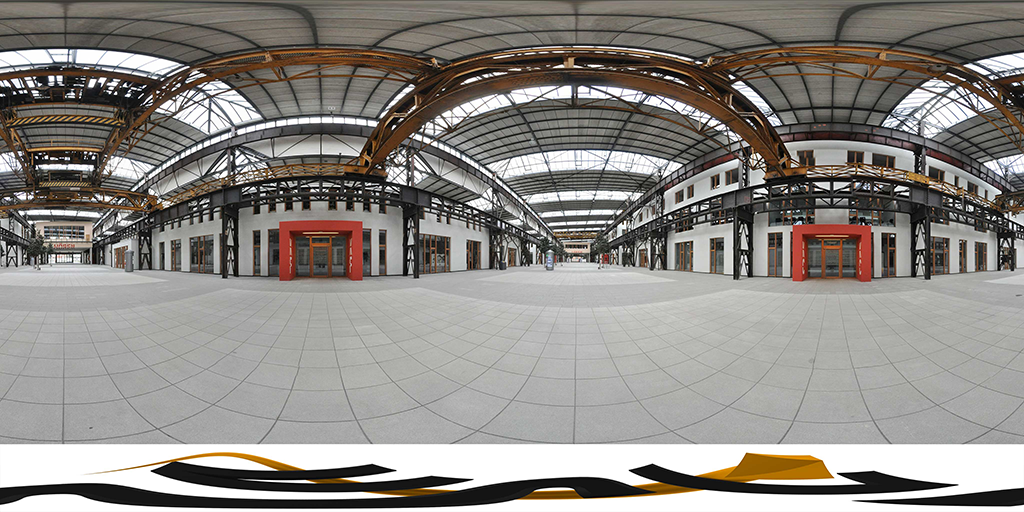
\includegraphics[width=0.8\textwidth]{Ueberarbeitet.png}
\caption[Panoramafoto nach Überarbeitung und Optimierung]{Panoramafoto nach
Überarbeitung und Optimierung\protect\footnotemark}
\label{fig:Ueberarbeitet}
\end{figure}
\footnotetext{Eigene Darstellung}

\paragraph{Aufteilung des Panoramafotos in Kacheln} \hfill \\

Das Blickfeld des Benutzers in der Anwendung nimmt immer nur einen Teil der
Rundumansicht ein. Somit kann auch immer nur ein Teil des Panoramafotos
dargestellt werden. Es ist daher nicht sinnvoll das komplette Panoramafoto in
der Anwendung zu laden, bevor es dem Benutzer präsentiert wird.
Aus diesem Grund wird das Panoramafoto in einem letzten Bearbeitungsschritt in
mehrere Kacheln aufgeteilt. Ziel dieser Aufteilung ist eine Steigerung der
Performanz und eine Reduzierung der Ladezeiten für die Panoramafotos in der
Anwendung. Es muss immer nur der Teil der Kacheln geladen werden, der dem
Benutzer aktuell präsentiert wird. Wenn sich das Blickfeld des Benutzers ändert,
können einzelne Kacheln schnell nachgeladen werden.

Die Aufteilung der Panoramafotos im Projekt erfolgt, wie auch die Überarbeitung
der Fotos, mit der Software Adobe Photoshop CS5. Auch hier kann die
Stapelverarbeitungsfunktion genutzt werden, um die Aufteilung der Panoramafotos
zu automatisieren.

\subsection{Softwareerstellung}
\label{sec:Softwareerstellung}

Die zu erstellende Software erfüllt die Anforderungen des Lastenheftes, in dem die Modelle und Konzepte der Entwurfsphase implementiert werden. Die Umsetzung eines solchen Projektes mit einem mehrköpfigem Projektteam erfordert neben entsprechenden Softwareentwürfen auch Vorbereitung und den Einsatz spezieller Entwicklungswerkzeuge (Tools), die im nachfolgenden Abschnitt beschrieben sind.

\subsubsection{Vorbereitung und Tools}
\label{sec:VorbereitungUndTools}

Die besondere Herausforderung des vorliegenden Projektes besteht darin, eine
mehrschichtige Software, bestehend aus Benutzer- und Administrationsansicht, in
einem Projektteam zu entwickeln, welches sich in zwei Punkten von der
Projektorganisation eines klassischen\footnotemark\ Softwareprojektes
unterscheidet. Zum einem muss  as Projektteam, bedingt durch unterschiedliche
Arbeitsorte, räumlich getrennt voneinander entwicklen können. Zum anderen
ist das Projektteam während des Entwicklungszeitraums nicht vollständig im
Projekt eingebunden. Es müssen Arbeits-, Urlaubs-, Prüfungs- und
Krankheitszeiten aller Mitglieder des Projektteams als hemmende Zeitfaktoren
berücksichtigt werden. Eine genauere Betrachtung dieser Projektsituation ist an
dieser Stelle nicht notwendig.

\footnotetext{Klassische Softwareprojekte werden hier als Projekte
in einer reinen Projektorganisation verstanden. Zur weiteren Vertiefung siehe
\citet[S.~105]{jenny2001}}

Die beiden genennten Aspekte bergen organisatorische Risiken und können auch zu
Problemen bei der Entwicklung führen. Das Hauptrisiko ist dabei ein Stillstand
des Projektes, welcher dadurch bedingt ist, dass alle Projektmitglieder auf das
Wissen eines Mitglieds angewiesen sind, welches gerade nicht zur Verfügung
steht. Dieses Risiko soll durch den Einsatz von zwei Entwicklungswerkzeugen
minimiert werden.

Zunächst muss dafür gesorgt werden, dass alle Mitglieder immer auf dem
aktuellen Stand des Projektes sind. Wird ein Entwicklungsschritt von einer
einzelnen Person abgeschlossen muss das Ergebnis den anderen zur Verfügung
gestellt werden. Zusätzlich müssen Änderungen am bestehnden Projektstand
kommentiert und dokumentiert werden. Diese Anforderung werden im vorliegenden
Projekt mithilfe einer Projektversionierung erreicht. Ein Versionierungstool
bietet hierbei die Möglichkeit den Quellcode eines Softwareprojektes zentral in
einem sogenannten Repository (zu deutsch "`Depot"') zu halten, um ihn für alle
Mitglieder verfübgar zu machen. Der aktuelle Stand des Projektes kann aus
diesem Repository jederzeit abgefragt werden und Änderungen werden von
Mitgliedern dorthin zurückgeschrieben. Zusätzlich bieten Versionierungstools die
Möglichkeit, die Änderung mit einem Kommentar zu versehen. Die Dokumentation der
konkrteten Änderungen wird vom Tool automatisch durchgeführt. Als
Versionierungssoftware wurde im vorliegenden Projekt "`Github"'\footnotemark\
verwendet, da allen Mitglieder mit diesem Versionierungstool bereits gearbeitet
haben.

\footnotetext{Github ist eine Open Source Projekt, das auf dem
Versionierungstool git aufsetzt. Es stellt den De-facto-Standard für
Webprojekte dar.}

Neben dem Quellcode sollen auch die Anforderungen an die Anwendung und die
aktuellen Aufgaben der Projektmitglieder an zentraler Stelle verwaltet werden.
Bei Ausfall eines Mitgliedes müssen seine aktuellen Aufgaben zentral
dokumentiert sein, um diese auf andere Mitglieder verteilen zu können. Dazu
wurde ein webbasiertes Ticketsystem aufgesetzt, auf das alle Mitglieder zugriff
haben. Hierbei wurde sich für das Ticketsystem "`PHProjekt"' entschieden, da PHP
als Technologie bereits bekannt ist und das Ticketsystem somit schnell
aufgesetzt werden konnte. In diesem Ticketsystem werden alle erstellten
Arbeitspakete des Projektes mit zugeordnetem Mitglied, Bearbeitungszeitraum,
Anforderungsbeschreibung und benötigter Bearbeitungszeit hinterlegt.
\subsubsection{Prototyp}
\label{sec:Prototyp}

Nach Bereitstellung des Ticketsystems und des Versionierungstools kann mit der Implementierung der Software begonnen werden. Für die Auftraggeber des Projektes war es dabei besonders wichtig, dass zunächst ein Prototyp der späteren Software entwickelt wird. Dieser Prototyp sollte nur die 360 Grad Ansicht eines Campus Panoramas und die Möglichkeit zu einem weiteren Panorama zu navigieren enthalten. Der Prototyp sollte genutzt werden um Entscheidungsträger von Beginn an vom Projekt zu überzeugen.

Da der Prototyp nur einen statischen Einblick (kein dynamischer Inhalt aus einer Datenbank) in die späteren Benutzeransicht gewähren sollte, wurde hierfür ein HTML-Dokument geschrieben, das die Google Street View API einbindet und über Javascript dessen Funktionalität implementiert. Das erstellte HTML-Dokument ist in \listing{HTML Prototyp} dargestellt:

\lstinputlisting[language=HTML,caption={HTML Prototyp},label={lst:HTML Prototyp}]{Listings/HTML_Prototyp.html}

Das dargestellte HTML-Dokument bindet in Zeile 5 die angesprochene Google Street View API, in der Funktionen zur Darstellung des 360 Grad Panoramas definiert sind. Zusätzlich wird in Zeile 6 eine Javascript-Datei eingebunden, in der die Funktionen der Google Street View API auferufen werden. Im Body-Bereich des HTML-Dokumentes ist dafür ein Element definiert das als Fläche zur Darstellung der Panoramas genutzt wird. Die eingebundene Javascript-Datei aus Zeile 6 ist aus Platzgründen in \listing{Javascript Prototyp} in Anhang ~\ref{sec:AnhangJavascriptPrototyp} dargestellt. Dessen Funktionalität wird an dieser Stelle kurz erläutert.
%TODO: Anhang XX richtig einfügen

Sobald der Internetbrowser des Benutzers das HTML-Dokument fertig geladen hat, wird eine Methode aufgerufen, die benötigte Parameter zur Erstellung des Panoramas bereitstellt\footnote{Vergleiche Zeile 3 im Anhang XX}. Hier werden Zoomstufe, Ausrichtung und weitere Parameter festgelegt. Anschließend wird ein Panorama-Objekt mit Hilfe der Google Street View API erstellt und an das oben beschriebene HTML-Element im Body-Bereich gebunden\footnote{Vergleiche Zeile 16-18 im Anhang XX}. Über einen weiteren Aufruf einer API-Funktion können an das Panorama sogenannte "`Links"' gehängt werden. Diese Links stellen später für den Benutzer die Pfeile am Boden dar über die zu anderen Panoramas navigiert werden kann. Im Prototyp wird nur der Verweis auf ein anderes Panorama gebraucht, das über die Funktion "`createCustomLinks"'\footnote{vergleiche Zeile 45ff. im Anhang XX} als Link angehängt wird.

Ein Bildschirmfoto des Prototypen der mitt diesen zwei Dateien (HTML- und Javascript-Dokument) erstellt wurde ist in \abbildung{PrototypScreenshot} zu sehen.

%TODO: Screenshot ohne Pixelfehler machen!
\begin{figure}[htb]
\centering

\includegraphics[width=1.0\textwidth]{PrototypScreenshot.png}
\caption[PrototypScreenshot]{Bildschirmfoto des Prototypen}
\label{fig:PrototypScreenshot}
\end{figure}
\subsubsection{Administrationsbereich}
\label{sec:UmsetzungAdministrationsbereich}

Der entwickelte Prototyp stellt eine erste lauffähige Version einer Benutzeransicht dar. Der nächste Entwicklungsschritt ist die Implementierung des Administrationsbereiche und die Bereitstellung von APIs. Aufbauend auf gepflegten Ìnformationen im Administrationsbereich wird der Prototyp dann um dynamische Funktionalität erweitert. Das heißt die angezeigten Panoramas und die benachbarten Panoramas werden über eine API angefragt, die die Informationen aus der Datenbank lädt. Der Implementierungsprozess des Administrationsbereiches wird dabei sukzessiv anhand der vorgestellten Anwendungsfällen (siehe \nameref{sec:Adminstratoranwendungen} auf Seite \pageref{sec:Adminstratoranwendungen}) realisiert. Prioresiert werden dabei die Anwendungsfälle, die die Verwaltung der Panoramas, Infotexte und die Übersichtskarte betreffen (AFA05 bis AFA17).

Bevor mit der Implementierung begonnen werden kann wird noch ein einheitliches Design festgelegt, dass vor allem dem späteren Administrator das Verständnis erleichtert. Zu diesem einheitlichen Design Konzept zählt zum Beispiel das Farbschema von Buttons. So wurde beispielsweise festgelegt, dass ein roter Button immer das Löschen eines Datensatzes signalisiert und ein grüner immer das speichern eines Datensatzes. Darüber hinaus wurde entschieden die Gestaltung von Buttons, Informationsfenster und ähnlichem mit dem CSS\footnotemark\ Framework Bootstrap\footnotemark\ zu realisieren. Dadurch ist gewährleistet, dass alle Steuerungselemente in allen Browsern gleich aussehen und der Administrator Elemente durch ihr Aussehen wiedererkennen und darüber auf ihre Benutzung schließen kann. Durch diese Entscheidungen wird die Usability der Software erhöht und der Aufwand der zu erstellenden Dokumentation verringert.

\footnotetext{CSS steht für Cascading Style Sheets und beschreibt eine Skriptsprache, die dazu dient HTML-Elemente in Form und Farbe zu verändern.}

\footnotetext{Bootstrap ist ein open Source Projekt, in dem einheitlich das Design von verschiedenen HTML-Elemente definiert ist. Bootstrap ist ein Projekt des Internetkonzerns Twitter und ist besonders dafür geeignet ein einheitliches Look and Feel einer Webseite in allen Browsern zu erzeugen.}

Aufbauend auf Administratoranwendungsfällen und Designkonzept werden Tickets erstellt, deren Inhalt die Implementierung der Infotext- und Fotoverwaltung ist. Zur Verdeutlichung der eingesetzten Technologien und des Entwicklunsablaufs wird im Folgenden eine stark vereinfachte Fotoverwaltungsseite implementiert. Implementiert werden soll eine Seite, die alle Fotos der Datenbank mit Namen und Beschreibung anzeigt. Zustätzlich soll es dem Administrator möglich sein auf den Namen eines Fotos zu klicken, woraufhin ihm weitere Informationen angezeigt werden.

Zur Implementierung dieses Szenarios wird zunächst ein HTML-Dokument angefertigt, dass das Grundgerüst der Fotoverwaltung darstellt. In diesem Grundgerüst könnten bestimmte Elemente, wie zum Beispiel die Navigationsbar am oberen Rand (vergleiche \abbildung{MockupBackend}) der Seite oder der Titel der Seite, statisch codiert werden. Zur Vereinfachung soll aber nur der Titel der Seite gesetzt werden und eine Überschrift. Das folgende \listing{HTML_Anwendungsbeispiel} zeigt das angefertigte HTML-Dokument.

\lstinputlisting[language=HTML,caption={statisches HTML},label={lst:HTML_Anwendungsbeispiel}]{Listings/HTML_Anwendungsbeispiel.html}

Im Anschluss daran muss die Seite um dynamisch generierten Inhalt erweitert werden. Dynamischer Inhalt ist im gegeben Anwendungsfall das Anzeigen aller Fotos, die bereits in der Datenbank sind. Um dieses Verhalten zu realisieren muss eine Anfrage an die Datenbank gestellt werden und danach muss für jeden Eintrag in der Datenbank HTML Quellcode geschrieben werden. Das nachfolgende \listing{HTML mit PHP} zeigt die Implementierung mit PHP.

\lstinputlisting[language=HTML,caption={Dynamisches schreiben von HTML mit PHP},label={lst:HTML mit PHP}]{Listings/HTML_mit_PHP.php}

Zu sehen ist die Anfrage an die Datenbank, die durch die PHP-Funktion "`mysql\_query"' (Zeile 5) realisiert wird, das Durchlaufen jeden Datenbanksatzes in einer Schleife (Zeile 6ff.) und das schreiben von HTML mit dem PHP "`echo"'-Befehl.

Zum Abschluss wird das klicken auf den Fotonamen implementiert. Diese Benutzerinteraktion kann am besten auf dem Clientsystem des Benutzers (Internetbrowser) mit Javascript verarbeitet werden, da keine weiteren Informationen vom Server benötigt werden und zusätzliche Anfragen so vermieden werden. Javascript-Routinen werden meistens als Funktionen formuliert, die aufgerufen werden, wenn ein bestimmtes Ereignis eintritt. Im \listing{HTML mit PHP} ist ein solcher Funktionsaufruf in Zeile 9 zu sehen. Die Funktion "`toggleDescription"' wird aufgerufen sobald auf das <p>-Tag geklickt wird. Als Parameter wird dieser Funktion das eigene HTML-Element, also das <p>-Tag, mitgegeben. Die Javascript-Funktion ist in \listing{Javascript Snippet} dargestellt.

\lstinputlisting[language=JavaScript,caption={Auf Benutzerinteraktion reagieren mit Javascript},label={lst:Javascript Snippet}]{Listings/Javascript_Snippet.js}

Alle dargestellten Listings könnten dabei in einem Dokument stehen, das vom dem Administrator über seinen Internetbrowser angefragt wird.
Wie bereits erwähnt ist diese Darstellung der Implementierung sehr stark vereinfacht. Die Quelldateien, die die Fotoverwaltung im vorliegenden Projekt implementieren, sind zu umfangreich, um sie an dieser Stelle zu präsentieren. Die implementierte Fotoverwaltung wird in folgendem Bildschirmfoto zur Veranschaulichung dargestellt:

%TODO: Bildschirmfoto ohne Pixelfehler machen.
\begin{figure}[htb]
\centering
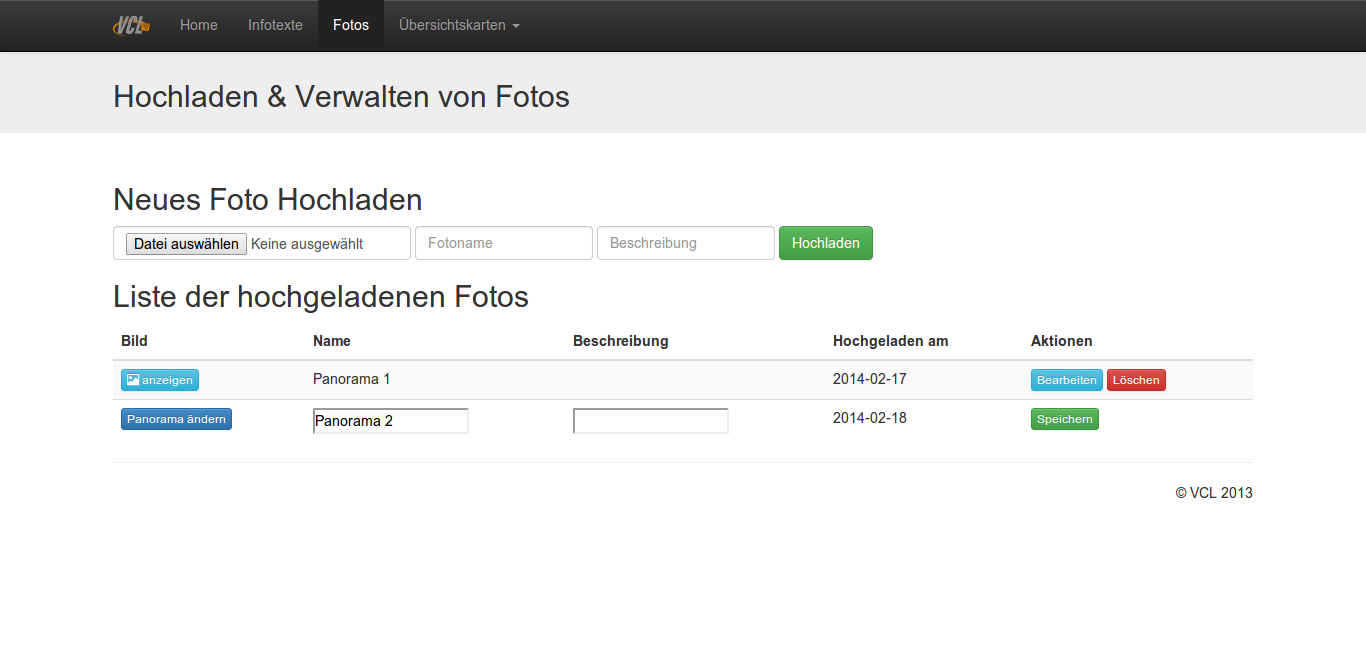
\includegraphics[width=1.0\textwidth]{Fotoverwaltung.png}
\caption[Fotoverwaltung]{Bildschirmfoto der implementierten Fotoverwaltung}
\label{fig:Fotoverwaltung}
\end{figure}

In einem solchen Entwicklungszyklus wurde auch die Verwaltung der Infotexte und die Übersichtskarte implementiert. Bildschirmfotos dieser Bereiche sind im Anhang dargstellt, siehe \abbildung{ScreenshotInfotext}, \abbildung{ScreenshotUebersichtskarte}.
\subsubsection{Application Programming Interfaces (APIs)}
\label{sec:APIs}

Aufbauend auf dem abgeschlossen Administrationsbereich werden im Folgenden
Application Programming Interfaces, kurz APIs, implementiert. Aufgabe solcher
APIs ist es, Informationen in maschinenleserlicher Form für andere Teilbereiche
des Systems bereitzustellen. Die bereitgestellten Informationen werden von den
aufrufenden Systemen genutzt, um Inhalte dynamisch darzustellen.
In einem Beispiel soll der zuvor vorgestellte Prototyp die Menge der
benachbarten Panoramas über eine solche API beziehen und darauf aufbauend dem
Benutzer die Navigationspfeile entsprechend präsentieren. Die Implementierung
einer API wird nachfolgend an diesem Beispiel erläutert.

Die Realisierung der Schnittstelle vollzieht sich in zwei Schritten.
Zuerst werden die Informationen maschienenleserlich geschrieben und ausgeben. Im
zweiten Schritt werden diese Informationen dann von einem verarbeitenden System
eingelesen und ausgewertet. Das Schreiben von maschinenleserlichen Informationen
hängt stark davon ab, welche Maschine den ausgegeben Text lesen bzw.
interpretieren soll. Im vorliegenden Projekt werden die erstellten APIs
ausschließlich von Javascript-Routinen angefragt, um Inhalte asynchron
nachzuladen. Auf die Bedeutung von asynchronem Nachladen wird später genauer
eingegangen. An dieser Stelle ist lediglich zu beachten, dass die APIs von
Javascript-Routinen angefragt werden. Aus diesem Grund werden die Informationen
der API im JSON-Format dargestellt. JSON steht dabei für "`Javascript Object
Notation"' und ist der de facto Standard für die Kommunikation zwischen
webbasierten Schnittstellen.\footnote{\citet[S.~20]{lubbers2011}} Die
Darstellung im JSON-Format bietet den großen Vorteil, dass innerhalb von
Javascript aus den dargestellten Informationen ein Objekt im Sinne der
objektorientierten Programmierung\footnotemark erstellt werden kann. An dieser
Stelle soll diese Begründung für die Wahl des JSON-Formats ausreichen. Eine
genauere Betrachtung erfolgt im zweiten Schritt der Implementierung der API.
Neben der Klassifikation der API muss noch der darzustellende Inhalt definiert
werden. Für den oben beschriebenen Anwendungsfall müssen hierbei alle Nachbarn
eines gegebenen Panoramas dargestellt werden. Für die Ausrichtung der
Navigationspfeile wird zusätzlich die Himmelsrichtung in Grad jedes Nachbarn
relativ zum Standpunkt des gegeben Panoramas benötigt. Dieser letzte Wert wird
als "`Heading"' bezeichnet und wird bereits bei der Positionierung des
360-Grad-Fotos in der Datenbank gespeichert. Er muss also nur aus der Datenbank
abgefragt werden.

\footnotetext{Die Objektorientierte Programmmierung (OOP) ist
das führende Programmierparadigma für Webanwendungen. Dieses Paradigma
beschreibt eine bestimmte Denkweise für Problemstellungen der Informatik. Für
weitere Einblicke siehe \citet{poetzsch2000}}

Aufbauend auf der vorausgegangenen Beschreibung der API kann diese in PHP
implementiert werden. Dazu wird zunächst das in \verweis{Datenbankentwurf}
beschriebene Tabellenmodell in Bezug auf die darzustellenden Informationen
untersucht. In der \abbildung{Tabellenmodell} ist zu sehen, dass
\textit{heading} ein Attribut der Tabelle \textit{neighbour} ist. Über diese
Tabelle können zu einem gegeben Panorama alle Nachbarn mit entsprechendem
\textit{heading} gefunden werden.
Im Zuge der Implementierung sollen im Folgenden mit Hilfe von PHP über SQL alle
Nachbarn eines gegebenen Panoramas abgefragt werden. Das Ergebnis dieser
Abfrage soll im JSON-Format dargestellt werden. Im \listing{PHP_Nachbar_API}
ist diese Funktionalität implementiert.

\lstinputlisting[language=PHP,caption={PHP Nachbar
API},label={lst:PHP_Nachbar_API}]{Listings/PHP_Nachbar_API.php}

Das gebene Panorama wird im Listing über die aufrufende URL, also einem
HTTP\footnotemark -Parameter, gesetzt. In der URL
\url{http://vcl.example.com/api/api\_test.php?id=1} würde beispielsweise der
Parameter id ("`?id=1"') mit der Panorama-ID 1 übergeben werden. Das
Auslesen dieser Information ist im Listing in Zeile 2 dargestellt.
Unter der Annahme, dass das Panorama mit der ID 1 zwei Nachbarn hat, würde der
Aufruf der API folgendes Ergebnis liefern:

\footnotetext{HTTP steht für Hypertext Transfer Protocol und bezeichnet ein
Protokoll, das den Übertragungsstandard für Webdokumente darstellt. HTTP stellt
damit eine fest protokollierte Struktur auf, in der geregelt ist, wie ein
Dokument über das Internet übertragen wird.}

\clearpage

\begin{figure}[htb]
\centering
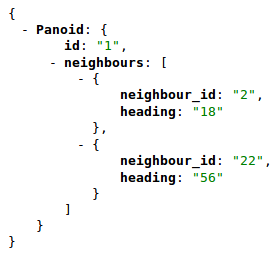
\includegraphics[width=0.4\textwidth]{ScreenshotAPIBeispiel.png}
\caption[API Beispiel]{Bildschirmfoto des gegebenen API Beispiels}
\label{fig:ScreenshotAPIBeispiel}
\end{figure}

Die Darstellung dieser Ausgabe wurde mit Hilfe eines Darstellungstools auf
bessere Lesbarkeit optimiert. Im Normalfall würde die Ausgabe in einer Zeile
dargestellt werden. Dies zeigt wiederum, dass das Ausgabeformat nicht auf
menschliche Lesbarkeit ausgelegt ist.

Nachdem das ausgebende System der Beispielschnittstelle implementiert wurde,
soll dieses nachfolgend angefragt und die Antwort des Systems ausgewertet
werden. Die Anfrage an das System erfolgt, wie bereits erwähnt, asynchron
innerhalb einer Javascript-Funktion. Asynchron bedeutet hierbei, dass die
Anfrage unabhängig von dem Aufbau der restlichen Seite ausgeführt wird.
Unabhängig von der aktuell dargestellten Seite wird eine Anfrage ausgeführt,
dessen Ergebnis in die bereits dargestellte Seite integriert wird.

In \verweis{Prototyp} wurde bereits die Funktion "`createCustomLink"' aus dem
Anhang ~\ref{sec:AnhangJavascriptPrototyp}
(\nameref{sec:AnhangJavascriptPrototyp}) vorgestellt. In dieser Funktion
werden die Links festgelegt, die letzenendes die Navigationspfeile in der
Benutzeransicht abbilden. Im \verweis{Prototyp} wurden diese Links statisch
gesetzt. Nachfolgend soll der Prototyp in der Weise abgeändert werden, dass die
Links durch Aufrufen der API dynamisch festgelegt werden. Dazu wird die Funktion
\textit{createCustomLink} zunächst um einen Funktionausruf der Funktion
"`getPanoJson"' erweitert. Diese Funktion ist dafür zuständig, die oben
definierte API mit einer übergebenen ID anzufragen und ein JSON-Objekt an die
aufrufende Methode zurückzuliefern. Die Implementierung dieser Funktion ist in
\listing{Dynamisch_Nachbarn_nachladen} dargestellt.

\clearpage

\lstinputlisting[language=JavaScript,caption={Dynamisch Nachbarn
nachladen},label={lst:Dynamisch_Nachbarn_nachladen}]{Listings/Dynamisch_Nachbarn_nachladen.js}

Die Funktion \textit{getPanoJson} wird in Zeile 5 aufgerufen und fragt daraufhin
über einen sogenannten \textit{XMLHttpRequest} die oben genannte URL an (Zeile
25). Da die Antwort als unformartiertes Textdokument erfolgt und es nicht
möglich ist per HTTP Objekte zu übertragen muss die Antwort zunächst in ein
JSON-Objekt umgewandelt werden. Man spricht dabei von "`parsen"' (Zeile 28). Die
Elemente des zurückgelieferten JSON-Objektes (Zeile 30) können daraufhin von der
aufrufenden Funktion referenziert werden. Über "`pano.neighbours"' (Zeile 7)
erhält man beispielsweise eine Liste aller Nachbarn, die im oben dargestellten
Quellcode durchlaufen und in die \textit{Links}-Liste geschrieben werden (Zeile
8ff.).

Durch die Erweiterung des Prototyps ist dieser in der Lage, die im
Administrationsbereich gepflegten Daten dynamisch abzurufen.

An dieser Stelle des Entwicklungsprozesses sind die Funktionen des
Administrationsbereichs vollständig umgesetzt und die Benutzeransicht greift
über APIs dynamisch auf die hinterlegten Informationen zu. Die Umsetzung des
Projektes ist damit abgeschlossen.
\subsubsection{Vorbereitung und Tools}
\label{sec:VorbereitungUndTools}

Die besondere Herausforderung des vorliegenden Projektes besteht darin, eine
mehrschichtige Software, bestehend aus Benutzer- und Administrationsansicht, in
einem Projektteam zu entwickeln, welches sich in zwei Punkten von der
Projektorganisation eines klassischen\footnotemark\ Softwareprojektes
unterscheidet. Zum einem muss  as Projektteam, bedingt durch unterschiedliche
Arbeitsorte, räumlich getrennt voneinander entwicklen können. Zum anderen
ist das Projektteam während des Entwicklungszeitraums nicht vollständig im
Projekt eingebunden. Es müssen Arbeits-, Urlaubs-, Prüfungs- und
Krankheitszeiten aller Mitglieder des Projektteams als hemmende Zeitfaktoren
berücksichtigt werden. Eine genauere Betrachtung dieser Projektsituation ist an
dieser Stelle nicht notwendig.

\footnotetext{Klassische Softwareprojekte werden hier als Projekte
in einer reinen Projektorganisation verstanden. Zur weiteren Vertiefung siehe
\citet[S.~105]{jenny2001}}

Die beiden genennten Aspekte bergen organisatorische Risiken und können auch zu
Problemen bei der Entwicklung führen. Das Hauptrisiko ist dabei ein Stillstand
des Projektes, welcher dadurch bedingt ist, dass alle Projektmitglieder auf das
Wissen eines Mitglieds angewiesen sind, welches gerade nicht zur Verfügung
steht. Dieses Risiko soll durch den Einsatz von zwei Entwicklungswerkzeugen
minimiert werden.

Zunächst muss dafür gesorgt werden, dass alle Mitglieder immer auf dem
aktuellen Stand des Projektes sind. Wird ein Entwicklungsschritt von einer
einzelnen Person abgeschlossen muss das Ergebnis den anderen zur Verfügung
gestellt werden. Zusätzlich müssen Änderungen am bestehnden Projektstand
kommentiert und dokumentiert werden. Diese Anforderung werden im vorliegenden
Projekt mithilfe einer Projektversionierung erreicht. Ein Versionierungstool
bietet hierbei die Möglichkeit den Quellcode eines Softwareprojektes zentral in
einem sogenannten Repository (zu deutsch "`Depot"') zu halten, um ihn für alle
Mitglieder verfübgar zu machen. Der aktuelle Stand des Projektes kann aus
diesem Repository jederzeit abgefragt werden und Änderungen werden von
Mitgliedern dorthin zurückgeschrieben. Zusätzlich bieten Versionierungstools die
Möglichkeit, die Änderung mit einem Kommentar zu versehen. Die Dokumentation der
konkrteten Änderungen wird vom Tool automatisch durchgeführt. Als
Versionierungssoftware wurde im vorliegenden Projekt "`Github"'\footnotemark\
verwendet, da allen Mitglieder mit diesem Versionierungstool bereits gearbeitet
haben.

\footnotetext{Github ist eine Open Source Projekt, das auf dem
Versionierungstool git aufsetzt. Es stellt den De-facto-Standard für
Webprojekte dar.}

Neben dem Quellcode sollen auch die Anforderungen an die Anwendung und die
aktuellen Aufgaben der Projektmitglieder an zentraler Stelle verwaltet werden.
Bei Ausfall eines Mitgliedes müssen seine aktuellen Aufgaben zentral
dokumentiert sein, um diese auf andere Mitglieder verteilen zu können. Dazu
wurde ein webbasiertes Ticketsystem aufgesetzt, auf das alle Mitglieder zugriff
haben. Hierbei wurde sich für das Ticketsystem "`PHProjekt"' entschieden, da PHP
als Technologie bereits bekannt ist und das Ticketsystem somit schnell
aufgesetzt werden konnte. In diesem Ticketsystem werden alle erstellten
Arbeitspakete des Projektes mit zugeordnetem Mitglied, Bearbeitungszeitraum,
Anforderungsbeschreibung und benötigter Bearbeitungszeit hinterlegt.
\subsubsection{Prototyp}
\label{sec:Prototyp}

Nach Bereitstellung des Ticketsystems und des Versionierungstools kann mit der Implementierung der Software begonnen werden. Für die Auftraggeber des Projektes war es dabei besonders wichtig, dass zunächst ein Prototyp der späteren Software entwickelt wird. Dieser Prototyp sollte nur die 360 Grad Ansicht eines Campus Panoramas und die Möglichkeit zu einem weiteren Panorama zu navigieren enthalten. Der Prototyp sollte genutzt werden um Entscheidungsträger von Beginn an vom Projekt zu überzeugen.

Da der Prototyp nur einen statischen Einblick (kein dynamischer Inhalt aus einer Datenbank) in die späteren Benutzeransicht gewähren sollte, wurde hierfür ein HTML-Dokument geschrieben, das die Google Street View API einbindet und über Javascript dessen Funktionalität implementiert. Das erstellte HTML-Dokument ist in \listing{HTML Prototyp} dargestellt:

\lstinputlisting[language=HTML,caption={HTML Prototyp},label={lst:HTML Prototyp}]{Listings/HTML_Prototyp.html}

Das dargestellte HTML-Dokument bindet in Zeile 5 die angesprochene Google Street View API, in der Funktionen zur Darstellung des 360 Grad Panoramas definiert sind. Zusätzlich wird in Zeile 6 eine Javascript-Datei eingebunden, in der die Funktionen der Google Street View API auferufen werden. Im Body-Bereich des HTML-Dokumentes ist dafür ein Element definiert das als Fläche zur Darstellung der Panoramas genutzt wird. Die eingebundene Javascript-Datei aus Zeile 6 ist aus Platzgründen in \listing{Javascript Prototyp} in Anhang ~\ref{sec:AnhangJavascriptPrototyp} dargestellt. Dessen Funktionalität wird an dieser Stelle kurz erläutert.
%TODO: Anhang XX richtig einfügen

Sobald der Internetbrowser des Benutzers das HTML-Dokument fertig geladen hat, wird eine Methode aufgerufen, die benötigte Parameter zur Erstellung des Panoramas bereitstellt\footnote{Vergleiche Zeile 3 im Anhang XX}. Hier werden Zoomstufe, Ausrichtung und weitere Parameter festgelegt. Anschließend wird ein Panorama-Objekt mit Hilfe der Google Street View API erstellt und an das oben beschriebene HTML-Element im Body-Bereich gebunden\footnote{Vergleiche Zeile 16-18 im Anhang XX}. Über einen weiteren Aufruf einer API-Funktion können an das Panorama sogenannte "`Links"' gehängt werden. Diese Links stellen später für den Benutzer die Pfeile am Boden dar über die zu anderen Panoramas navigiert werden kann. Im Prototyp wird nur der Verweis auf ein anderes Panorama gebraucht, das über die Funktion "`createCustomLinks"'\footnote{vergleiche Zeile 45ff. im Anhang XX} als Link angehängt wird.

Ein Bildschirmfoto des Prototypen der mitt diesen zwei Dateien (HTML- und Javascript-Dokument) erstellt wurde ist in \abbildung{PrototypScreenshot} zu sehen.

%TODO: Screenshot ohne Pixelfehler machen!
\begin{figure}[htb]
\centering

\includegraphics[width=1.0\textwidth]{PrototypScreenshot.png}
\caption[PrototypScreenshot]{Bildschirmfoto des Prototypen}
\label{fig:PrototypScreenshot}
\end{figure}
\subsubsection{Administrationsbereich}
\label{sec:UmsetzungAdministrationsbereich}

Der entwickelte Prototyp stellt eine erste lauffähige Version einer Benutzeransicht dar. Der nächste Entwicklungsschritt ist die Implementierung des Administrationsbereiche und die Bereitstellung von APIs. Aufbauend auf gepflegten Ìnformationen im Administrationsbereich wird der Prototyp dann um dynamische Funktionalität erweitert. Das heißt die angezeigten Panoramas und die benachbarten Panoramas werden über eine API angefragt, die die Informationen aus der Datenbank lädt. Der Implementierungsprozess des Administrationsbereiches wird dabei sukzessiv anhand der vorgestellten Anwendungsfällen (siehe \nameref{sec:Adminstratoranwendungen} auf Seite \pageref{sec:Adminstratoranwendungen}) realisiert. Prioresiert werden dabei die Anwendungsfälle, die die Verwaltung der Panoramas, Infotexte und die Übersichtskarte betreffen (AFA05 bis AFA17).

Bevor mit der Implementierung begonnen werden kann wird noch ein einheitliches Design festgelegt, dass vor allem dem späteren Administrator das Verständnis erleichtert. Zu diesem einheitlichen Design Konzept zählt zum Beispiel das Farbschema von Buttons. So wurde beispielsweise festgelegt, dass ein roter Button immer das Löschen eines Datensatzes signalisiert und ein grüner immer das speichern eines Datensatzes. Darüber hinaus wurde entschieden die Gestaltung von Buttons, Informationsfenster und ähnlichem mit dem CSS\footnotemark\ Framework Bootstrap\footnotemark\ zu realisieren. Dadurch ist gewährleistet, dass alle Steuerungselemente in allen Browsern gleich aussehen und der Administrator Elemente durch ihr Aussehen wiedererkennen und darüber auf ihre Benutzung schließen kann. Durch diese Entscheidungen wird die Usability der Software erhöht und der Aufwand der zu erstellenden Dokumentation verringert.

\footnotetext{CSS steht für Cascading Style Sheets und beschreibt eine Skriptsprache, die dazu dient HTML-Elemente in Form und Farbe zu verändern.}

\footnotetext{Bootstrap ist ein open Source Projekt, in dem einheitlich das Design von verschiedenen HTML-Elemente definiert ist. Bootstrap ist ein Projekt des Internetkonzerns Twitter und ist besonders dafür geeignet ein einheitliches Look and Feel einer Webseite in allen Browsern zu erzeugen.}

Aufbauend auf Administratoranwendungsfällen und Designkonzept werden Tickets erstellt, deren Inhalt die Implementierung der Infotext- und Fotoverwaltung ist. Zur Verdeutlichung der eingesetzten Technologien und des Entwicklunsablaufs wird im Folgenden eine stark vereinfachte Fotoverwaltungsseite implementiert. Implementiert werden soll eine Seite, die alle Fotos der Datenbank mit Namen und Beschreibung anzeigt. Zustätzlich soll es dem Administrator möglich sein auf den Namen eines Fotos zu klicken, woraufhin ihm weitere Informationen angezeigt werden.

Zur Implementierung dieses Szenarios wird zunächst ein HTML-Dokument angefertigt, dass das Grundgerüst der Fotoverwaltung darstellt. In diesem Grundgerüst könnten bestimmte Elemente, wie zum Beispiel die Navigationsbar am oberen Rand (vergleiche \abbildung{MockupBackend}) der Seite oder der Titel der Seite, statisch codiert werden. Zur Vereinfachung soll aber nur der Titel der Seite gesetzt werden und eine Überschrift. Das folgende \listing{HTML_Anwendungsbeispiel} zeigt das angefertigte HTML-Dokument.

\lstinputlisting[language=HTML,caption={statisches HTML},label={lst:HTML_Anwendungsbeispiel}]{Listings/HTML_Anwendungsbeispiel.html}

Im Anschluss daran muss die Seite um dynamisch generierten Inhalt erweitert werden. Dynamischer Inhalt ist im gegeben Anwendungsfall das Anzeigen aller Fotos, die bereits in der Datenbank sind. Um dieses Verhalten zu realisieren muss eine Anfrage an die Datenbank gestellt werden und danach muss für jeden Eintrag in der Datenbank HTML Quellcode geschrieben werden. Das nachfolgende \listing{HTML mit PHP} zeigt die Implementierung mit PHP.

\lstinputlisting[language=HTML,caption={Dynamisches schreiben von HTML mit PHP},label={lst:HTML mit PHP}]{Listings/HTML_mit_PHP.php}

Zu sehen ist die Anfrage an die Datenbank, die durch die PHP-Funktion "`mysql\_query"' (Zeile 5) realisiert wird, das Durchlaufen jeden Datenbanksatzes in einer Schleife (Zeile 6ff.) und das schreiben von HTML mit dem PHP "`echo"'-Befehl.

Zum Abschluss wird das klicken auf den Fotonamen implementiert. Diese Benutzerinteraktion kann am besten auf dem Clientsystem des Benutzers (Internetbrowser) mit Javascript verarbeitet werden, da keine weiteren Informationen vom Server benötigt werden und zusätzliche Anfragen so vermieden werden. Javascript-Routinen werden meistens als Funktionen formuliert, die aufgerufen werden, wenn ein bestimmtes Ereignis eintritt. Im \listing{HTML mit PHP} ist ein solcher Funktionsaufruf in Zeile 9 zu sehen. Die Funktion "`toggleDescription"' wird aufgerufen sobald auf das <p>-Tag geklickt wird. Als Parameter wird dieser Funktion das eigene HTML-Element, also das <p>-Tag, mitgegeben. Die Javascript-Funktion ist in \listing{Javascript Snippet} dargestellt.

\lstinputlisting[language=JavaScript,caption={Auf Benutzerinteraktion reagieren mit Javascript},label={lst:Javascript Snippet}]{Listings/Javascript_Snippet.js}

Alle dargestellten Listings könnten dabei in einem Dokument stehen, das vom dem Administrator über seinen Internetbrowser angefragt wird.
Wie bereits erwähnt ist diese Darstellung der Implementierung sehr stark vereinfacht. Die Quelldateien, die die Fotoverwaltung im vorliegenden Projekt implementieren, sind zu umfangreich, um sie an dieser Stelle zu präsentieren. Die implementierte Fotoverwaltung wird in folgendem Bildschirmfoto zur Veranschaulichung dargestellt:

%TODO: Bildschirmfoto ohne Pixelfehler machen.
\begin{figure}[htb]
\centering
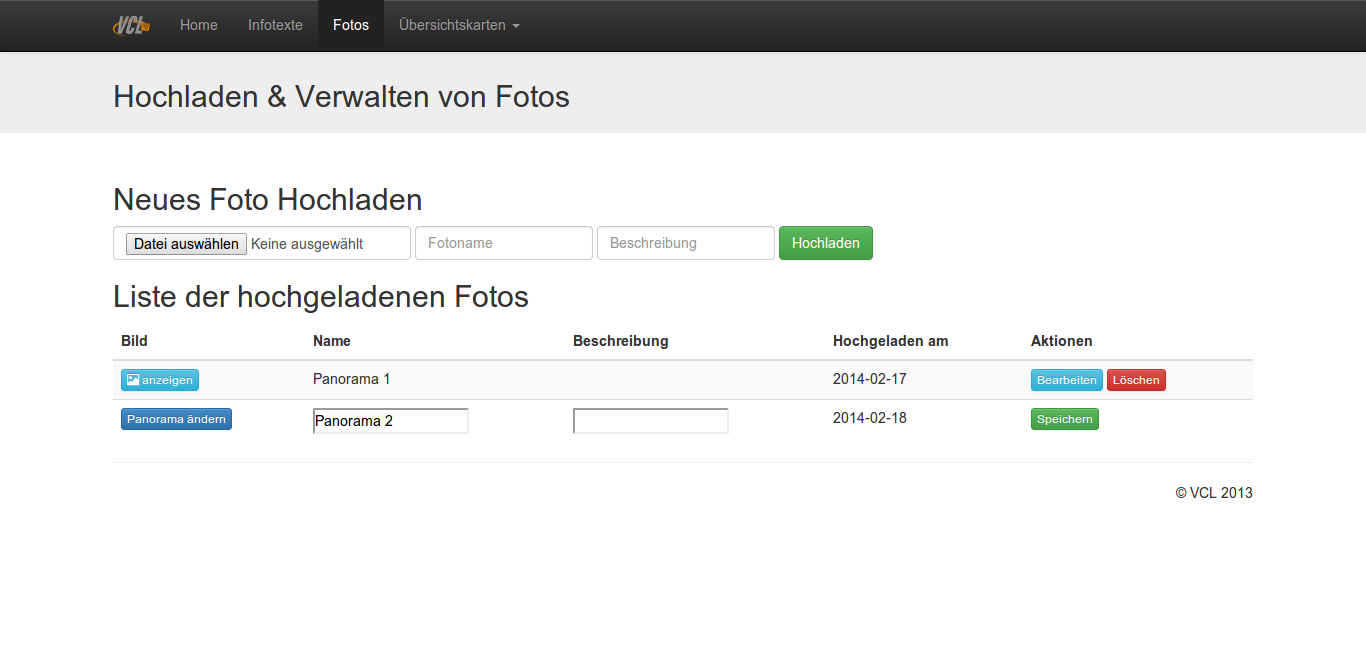
\includegraphics[width=1.0\textwidth]{Fotoverwaltung.png}
\caption[Fotoverwaltung]{Bildschirmfoto der implementierten Fotoverwaltung}
\label{fig:Fotoverwaltung}
\end{figure}

In einem solchen Entwicklungszyklus wurde auch die Verwaltung der Infotexte und die Übersichtskarte implementiert. Bildschirmfotos dieser Bereiche sind im Anhang dargstellt, siehe \abbildung{ScreenshotInfotext}, \abbildung{ScreenshotUebersichtskarte}.
\subsubsection{Application Programming Interfaces (APIs)}
\label{sec:APIs}

Aufbauend auf dem abgeschlossen Administrationsbereich werden im Folgenden
Application Programming Interfaces, kurz APIs, implementiert. Aufgabe solcher
APIs ist es, Informationen in maschinenleserlicher Form für andere Teilbereiche
des Systems bereitzustellen. Die bereitgestellten Informationen werden von den
aufrufenden Systemen genutzt, um Inhalte dynamisch darzustellen.
In einem Beispiel soll der zuvor vorgestellte Prototyp die Menge der
benachbarten Panoramas über eine solche API beziehen und darauf aufbauend dem
Benutzer die Navigationspfeile entsprechend präsentieren. Die Implementierung
einer API wird nachfolgend an diesem Beispiel erläutert.

Die Realisierung der Schnittstelle vollzieht sich in zwei Schritten.
Zuerst werden die Informationen maschienenleserlich geschrieben und ausgeben. Im
zweiten Schritt werden diese Informationen dann von einem verarbeitenden System
eingelesen und ausgewertet. Das Schreiben von maschinenleserlichen Informationen
hängt stark davon ab, welche Maschine den ausgegeben Text lesen bzw.
interpretieren soll. Im vorliegenden Projekt werden die erstellten APIs
ausschließlich von Javascript-Routinen angefragt, um Inhalte asynchron
nachzuladen. Auf die Bedeutung von asynchronem Nachladen wird später genauer
eingegangen. An dieser Stelle ist lediglich zu beachten, dass die APIs von
Javascript-Routinen angefragt werden. Aus diesem Grund werden die Informationen
der API im JSON-Format dargestellt. JSON steht dabei für "`Javascript Object
Notation"' und ist der de facto Standard für die Kommunikation zwischen
webbasierten Schnittstellen.\footnote{\citet[S.~20]{lubbers2011}} Die
Darstellung im JSON-Format bietet den großen Vorteil, dass innerhalb von
Javascript aus den dargestellten Informationen ein Objekt im Sinne der
objektorientierten Programmierung\footnotemark erstellt werden kann. An dieser
Stelle soll diese Begründung für die Wahl des JSON-Formats ausreichen. Eine
genauere Betrachtung erfolgt im zweiten Schritt der Implementierung der API.
Neben der Klassifikation der API muss noch der darzustellende Inhalt definiert
werden. Für den oben beschriebenen Anwendungsfall müssen hierbei alle Nachbarn
eines gegebenen Panoramas dargestellt werden. Für die Ausrichtung der
Navigationspfeile wird zusätzlich die Himmelsrichtung in Grad jedes Nachbarn
relativ zum Standpunkt des gegeben Panoramas benötigt. Dieser letzte Wert wird
als "`Heading"' bezeichnet und wird bereits bei der Positionierung des
360-Grad-Fotos in der Datenbank gespeichert. Er muss also nur aus der Datenbank
abgefragt werden.

\footnotetext{Die Objektorientierte Programmmierung (OOP) ist
das führende Programmierparadigma für Webanwendungen. Dieses Paradigma
beschreibt eine bestimmte Denkweise für Problemstellungen der Informatik. Für
weitere Einblicke siehe \citet{poetzsch2000}}

Aufbauend auf der vorausgegangenen Beschreibung der API kann diese in PHP
implementiert werden. Dazu wird zunächst das in \verweis{Datenbankentwurf}
beschriebene Tabellenmodell in Bezug auf die darzustellenden Informationen
untersucht. In der \abbildung{Tabellenmodell} ist zu sehen, dass
\textit{heading} ein Attribut der Tabelle \textit{neighbour} ist. Über diese
Tabelle können zu einem gegeben Panorama alle Nachbarn mit entsprechendem
\textit{heading} gefunden werden.
Im Zuge der Implementierung sollen im Folgenden mit Hilfe von PHP über SQL alle
Nachbarn eines gegebenen Panoramas abgefragt werden. Das Ergebnis dieser
Abfrage soll im JSON-Format dargestellt werden. Im \listing{PHP_Nachbar_API}
ist diese Funktionalität implementiert.

\lstinputlisting[language=PHP,caption={PHP Nachbar
API},label={lst:PHP_Nachbar_API}]{Listings/PHP_Nachbar_API.php}

Das gebene Panorama wird im Listing über die aufrufende URL, also einem
HTTP\footnotemark -Parameter, gesetzt. In der URL
\url{http://vcl.example.com/api/api\_test.php?id=1} würde beispielsweise der
Parameter id ("`?id=1"') mit der Panorama-ID 1 übergeben werden. Das
Auslesen dieser Information ist im Listing in Zeile 2 dargestellt.
Unter der Annahme, dass das Panorama mit der ID 1 zwei Nachbarn hat, würde der
Aufruf der API folgendes Ergebnis liefern:

\footnotetext{HTTP steht für Hypertext Transfer Protocol und bezeichnet ein
Protokoll, das den Übertragungsstandard für Webdokumente darstellt. HTTP stellt
damit eine fest protokollierte Struktur auf, in der geregelt ist, wie ein
Dokument über das Internet übertragen wird.}

\clearpage

\begin{figure}[htb]
\centering
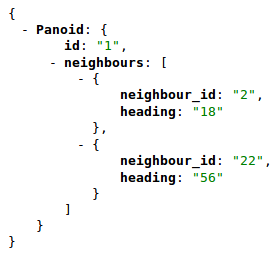
\includegraphics[width=0.4\textwidth]{ScreenshotAPIBeispiel.png}
\caption[API Beispiel]{Bildschirmfoto des gegebenen API Beispiels}
\label{fig:ScreenshotAPIBeispiel}
\end{figure}

Die Darstellung dieser Ausgabe wurde mit Hilfe eines Darstellungstools auf
bessere Lesbarkeit optimiert. Im Normalfall würde die Ausgabe in einer Zeile
dargestellt werden. Dies zeigt wiederum, dass das Ausgabeformat nicht auf
menschliche Lesbarkeit ausgelegt ist.

Nachdem das ausgebende System der Beispielschnittstelle implementiert wurde,
soll dieses nachfolgend angefragt und die Antwort des Systems ausgewertet
werden. Die Anfrage an das System erfolgt, wie bereits erwähnt, asynchron
innerhalb einer Javascript-Funktion. Asynchron bedeutet hierbei, dass die
Anfrage unabhängig von dem Aufbau der restlichen Seite ausgeführt wird.
Unabhängig von der aktuell dargestellten Seite wird eine Anfrage ausgeführt,
dessen Ergebnis in die bereits dargestellte Seite integriert wird.

In \verweis{Prototyp} wurde bereits die Funktion "`createCustomLink"' aus dem
Anhang ~\ref{sec:AnhangJavascriptPrototyp}
(\nameref{sec:AnhangJavascriptPrototyp}) vorgestellt. In dieser Funktion
werden die Links festgelegt, die letzenendes die Navigationspfeile in der
Benutzeransicht abbilden. Im \verweis{Prototyp} wurden diese Links statisch
gesetzt. Nachfolgend soll der Prototyp in der Weise abgeändert werden, dass die
Links durch Aufrufen der API dynamisch festgelegt werden. Dazu wird die Funktion
\textit{createCustomLink} zunächst um einen Funktionausruf der Funktion
"`getPanoJson"' erweitert. Diese Funktion ist dafür zuständig, die oben
definierte API mit einer übergebenen ID anzufragen und ein JSON-Objekt an die
aufrufende Methode zurückzuliefern. Die Implementierung dieser Funktion ist in
\listing{Dynamisch_Nachbarn_nachladen} dargestellt.

\clearpage

\lstinputlisting[language=JavaScript,caption={Dynamisch Nachbarn
nachladen},label={lst:Dynamisch_Nachbarn_nachladen}]{Listings/Dynamisch_Nachbarn_nachladen.js}

Die Funktion \textit{getPanoJson} wird in Zeile 5 aufgerufen und fragt daraufhin
über einen sogenannten \textit{XMLHttpRequest} die oben genannte URL an (Zeile
25). Da die Antwort als unformartiertes Textdokument erfolgt und es nicht
möglich ist per HTTP Objekte zu übertragen muss die Antwort zunächst in ein
JSON-Objekt umgewandelt werden. Man spricht dabei von "`parsen"' (Zeile 28). Die
Elemente des zurückgelieferten JSON-Objektes (Zeile 30) können daraufhin von der
aufrufenden Funktion referenziert werden. Über "`pano.neighbours"' (Zeile 7)
erhält man beispielsweise eine Liste aller Nachbarn, die im oben dargestellten
Quellcode durchlaufen und in die \textit{Links}-Liste geschrieben werden (Zeile
8ff.).

Durch die Erweiterung des Prototyps ist dieser in der Lage, die im
Administrationsbereich gepflegten Daten dynamisch abzurufen.

An dieser Stelle des Entwicklungsprozesses sind die Funktionen des
Administrationsbereichs vollständig umgesetzt und die Benutzeransicht greift
über APIs dynamisch auf die hinterlegten Informationen zu. Die Umsetzung des
Projektes ist damit abgeschlossen.

\section{Test}
\section{Projektabschluss}
\subsection{Dokumentation}
\subsection{Übergabe}
\section{Ausblick}
\section{Fazit}
\section{Kritische Reflexion}